\chapter{Pithos Evaluation}
    \label{chp:EVALUATION}

Following the discussion of the Pithos design and implementation, the performance of Pithos will now be presented, along with a comparison of Pithos against overlay storage.

Section \ref{key_mechanisms} presents the key mechanisms that Pithos uses to enable it to satisfy the goals set out in Section \ref{use_cases_goals}. Section \ref{key_mechanisms} often describes multiple methods in which a mechanism is implemented. The reason for implementing mechanisms using multiple methods is to enable their comparison. Some methods are theoretically better than others, while some methods are better suited to differing network conditions.

The purpose of this chapter is twofold. To compare the various methods of mechanism implementation and to compare Pithos with other storage architectures reviewed in Chapter \ref{p2p_MMVE_state_persistency}. Each comparison will be performed using the applicable metrics defined in Section \ref{key_challenges_cm}. All metrics were also measured as described in that section, but specific measurement details, as it relates to the simulation implementation will also be presented in this chapter.

\section{Simulation setup}
\label{simulation_setup}

In the results shown, Chord was used as the P2P overlay, mainly due to its faster simulation time, compared to Pastry. Pithos has, however, also been tested with Pastry and results are similar.

After a node has joined the network, PithosTestApp starts to generate store and retrieve requests at a rate of one objects every 5 seconds for a total of 20s and a size of 1024 bytes. The size of 1024 byte objects was chosen to be much larger than Quake 3 game objects without delta encoding, used in \cite{Bharambe_Donnybrook}. Pithos is designed for the low latency storage of small game objects. The limit of 20s generation time for every new peer joining the network is to reduce the memory required to store all objects. With the current setup, every simulation run requires 6 gigabytes of memory.

%The node lifetime should still be justified
For the results shown, 2500 peers, 100 super peers and a single directory server are created at the start of the simulation. The simulation runs for 10,000 seconds. Exponential node lifetimes are used when testing the store and retrieve requests. The applicability of this lifetime distribution will be explored in Section \ref{}. The Pithos simulation has also been successfully evaluated using Pareto lifetime distributions, another common distribution in reliability engineering. For the results presented here, the exponential distribution was used, due to its constant hazard rate \cite{}.

The overlay storage module stores 4 object replicas and always requests 4 replicas in parallel, similar to Pithos's parallel retrieval. Overlay storage expects the majority of requests to be identical, before success is reported. The remaining overlay setup parameters are discussed in Section \ref{overlay_resp_rel_results}.

The simulation uses a channel bandwidth of 10 Mbps. Pithos has also been successfully tested for a 1 Mbps link. Results of the 1 Mbps link are similar to the 10 Mbps results. The bandwidth requirements of Pithos is also evaluated in this chapter.

\section{Storage and retrieval performance}

Firstly, the storage and retrieval performance of Pithos and overlay storage are evaluated. The purpose of this section is to establish the baseline of Pithos performance under a basic simulation setup. Therefore, no object repair is performed and no malicious users exist. The network, however, still contains churn.

\subsection{Experimental setup}
\label{store_retrieve_exp_setup}

To evaluate storage and retrieval performance, nodes with 1800s mean lifetimes are used. This is much less than 615 min (36900s) mean playing time measured in WoW \cite{wow_gameplay}, but if the systems performs acceptably under the higher churn rate, it can only perform better for lower churn rates. The effect of churn on the network will be evaluated in Section \ref{repair_results}.

The results presented in Tables \ref{tab_pithos_storage_results} and \ref{tab_pithos_retrieval_results} are for a medium overlay storage configuration as described in Section \ref{overlay_resp_rel_results} and for 100\% group probability, as described in Section \ref{group_probability_results}.

Every object is stored with a TTL of 300s. The low TTL, compared to the expected node lifetime (1800s), is to ensure object survival with high probability in the absence of repair.

\subsection{Pithos reliability and responsiveness}
\label{pithos_resp_rel_results}

Tables \ref{tab_pithos_storage_results} and \ref{tab_pithos_retrieval_results} present the reliability and responsiveness results for the various Pithos storage and retrieval methods discussed in Sections \ref{store_implementation} and \ref{retrieve_implementation}.
Both safe and fast storage and fast and parallel retrieval are compared. Safe retrieval will be evaluated in Section \ref{malicious_results}. It should be noted that because Pithos is a group/overlay hybrid storage, its performance depends on the underlying group and overlay performance.

It does not make sense to evaluate retrieval performance apart from the storage method used, since the storage method will influence the retrieval method results as will be explained. Therefore, for each storage method in table \ref{tab_pithos_rel_resp_results}, it firstly shows the performance of only the specific storage method. The retrieval performance is then evaluated, taking into account the storage method used.

\subsubsection{Storage}
\begin{table}[htbp]
\centering
\begin{tabular}{|c|c|c|}
\hline
Storage method & Reliability & Responsiveness (s)\\
\hline
Safe    &  0.9705  &   1.554  \\
Fast    &  1.0     &   0.0488 \\
\hline
\end{tabular}
\caption{Responsiveness and reliability of Pithos's safe and fast storage.}
\label{tab_pithos_storage_results}
\end{table}
%
Table \ref{tab_pithos_storage_results} shows that when fast storage is used, a reliability of 1.0 is achieved, which is higher then the 0.970 reliability of sage storage. The real reliability isn't actually higher, but because fast storage only waits for a single successful response before reporting success, it reports more successful storages. Safe storage, on the other hand, ensures that a majority of replicas were successfully stored before reporting success. Fast storage will still report success, even if the majority of files were not successfully stored.

The advantage of fast storage over safe storage is its higher responsiveness of 0.0488 s, compared to safe storage's 1.576 s. This means that data are available for retrieval 32 times faster with fast storage compared to safe storage.

\subsubsection{Retrieval}

\begin{table}[htbp]
\centering
\begin{tabular}{|c|c|c|c|}
\hline
Storage method & Retrieval method & Reliability & Responsiveness (s)\\
\hline
Safe    &   Fast        &   0.9977  &   0.189  \\
Safe    &   Parallel    &   0.9998  &   0.0859 \\
Fast    &   Fast        &   0.9970  &   0.192  \\
Fast    &   Parallel    &   0.9998  &   0.0846 \\
\hline
\end{tabular}
\caption{Responsiveness and reliability of fast and parallel retrieval for safe and fast storage.}
\label{tab_pithos_retrieval_results}
\end{table}
%
Figure \ref{tab_pithos_retrieval_results} shows the results of fast and parallel retrieval for fast and safe storage respectively. Fast retrieval for fast storage performs worse (0.9970) than fast retrieval for safe storage (0.9977), but only marginally so. It performs worse, because objects that were incorrectly reported as successfully stored by fast storage, was in fact not. When fast retrieval attempts to retrieve an object stored with fewer replicas, there is a good chance that the object has been destroyed and the request is unsuccessful.

The same is true for parallel retrieval for fast storage, compared to parallel retrieval for safe storage. Safe storage leads to an increase in retrieval reliability at the cost of longer storage times.

Comparing parallel retrieval for fast storage to fast retrieval for fast storage leads to similar results as the comparison of parallel retrieval for safe storage to fast retrieval of safe storage. Parallel retrieval is both more reliable and responsive than fast retrieval. Parallel retrieval (0.9998) is more reliable than fast retrieval (0.9970), because of more requests being sent, which increases the probability that the request arrives at a node that is not about the leave the network.

The responsiveness of parallel retrieval (0.0876 s) is also higher than fast retrieval (0.196 s), because fast retrieval uses the first received response. The responsiveness of a retrieval request depends only on the fastest received response. If more retrieval requests are sent, the expected response time decreases because more links are now used. In other words, if more links are used, there is a higher probability of at least one link being faster than the others.

It should be noted that the Pithos responsiveness is highly dependant on the underlying network performance. The fast storage, fast retrieval performance of 192ms might seem slow, but is a function of the connectedness and responsiveness of the underlying links. In the Oversim case, the underlying link properties are represented by the SimpleUnderlayNetwork, as described in Section \ref{oversim_underlay}.

The SimpleUnderlayNetwork is a global scale network, which means that the Pithos responsiveness should be seen in the context of operating in a network distributed across the world. What will be of use is to see what the Pithos performance is, for fixed network responsiveness in a local area network (LAN) environment. This is presented in Section \ref{lan_retrieval}.

For the Pithos implementation, fast storage has been adopted as the norm, over safe storage. The factor 32 increase in responsiveness is seen to outweigh the factor 1.029 decrease in performance.

The question whether fast or parallel retrieval is preferred depends on the implementation environment. Fast retrieval does not allow for malicious nodes in the network, since fast retrieval sends the first received object to the higher layer. This leaves no time to compare objects received from multiple nodes. To be able to better compare fast retrieval with parallel retrieval, the bandwidth requirements of the two methods should also be compared.

\subsection{Overlay reliability and responsiveness}
\label{overlay_resp_rel_results}

For overlay storage, the three configurations represent high, medium and low levels of reliability and bandwidth requirements respectively. The main parameter modified to achieve these varying levels of responsiveness and reliability is the Chord finger table update time. The update time determines how up-to-date the Chord finger tables are and by extension, how up to date Chord's view of the network is.

Table \ref{tab_overlay_medium} shows the ``medium'' overlay configuration parameters and their values:
%
\begin{table}[htbp]
\centering
\begin{tabular}{|r|l|l|l|}
\hline
Parameter                       & Low  & Medium & High  \\
\hline
Stabilise retries               & 1    & 2      &  3    \\
Stabilise delay                 & 10s  & 5s     &  3s   \\
Fix finger table interval       & 120s & 10s    &  5s   \\
Check predecessor delay         & 5s   & 5 s    &  3s   \\
Extended finger table           & no   & yes    &  yes  \\
Extended finger table candidate & N/A  & 3      &  4    \\
\hline
\end{tabular}
\caption{Overlay storage medium configuration parameters and values.}
\label{tab_overlay_configs}
\end{table}

Table \ref{tab_overlay_configs} shows the ``low'', ``medium'' and ``high'' overlay configuration parameters and their values. These are the overlay configurations that were used during the testing of Pithos and its comparison with overlay storage.

The purpose of the ``high'' configuration is to match the Pithos reliability performance and to then compare overlay responsiveness and bandwidth usage with that of Pithos. This setup was achieved by itteratively adjusting the Chord parameters until similar reliability to that of Pithos was achieved.

Table \ref{tab_overlay_rel_resp_results} shows the responsiveness of overlay storage for the various parameter settings as described earlier in this section. Because of how the settings were defined, high has the highest storage reliability of 0.9831, medium has a storage reliability of 0.969 and low has the lowest storage reliablity of 0.7908. High also possesses the higher retrieval reliability of 0.9365, medium has a retrieval reliability of 0.9320 and low has the lowest retrieval reliability of 0.6216.
%
\begin{table}[htbp]
\centering
\begin{tabular}{|c|c|c|c|c|}
\hline
Configuration type & Reliability & Responsiveness (s)\\
\hline
High storage     &   0.9831      &   1.217  \\
High retrieval   &   0.9365      &   1.745  \\
Medium storage   &   0.969       &   1.214  \\
Medium retrieval &   0.9320      &   1.582  \\
Low storage      &   0.7908      &   1.245  \\
Low retrieval    &   0.6216      &   2.071  \\
\hline
\end{tabular}
\caption{Evaluation of overlay storage responsiveness and reliability for various Chord parameter settings.}
\label{tab_overlay_rel_resp_results}
\end{table}

What is also clear from Table \ref{tab_overlay_rel_resp_results} is that the less reliable the storage, the longer it takes to retrieve an item, which further amplifies the importance of high overlay reliability.

\subsection{Bandwidth requirements}
\label{bandwidth_requirements}

\begin{table}[htbp]
\centering
\begin{tabular}{|c|c|c|c|}
\hline
Entity & Storage method & Retrieval method     & Bandwidth\\
       &                &                      & in/out (Bps)\\
\hline
Group   &   Fast        &   Fast               &   187/183\\
Group   &   Safe        &   Fast               &   183/180\\
Group   &   Safe        &   Parallel           &   798/749\\
Group   &   Fast        &   Parallel           &   784/735\\
\hline
Overlay &   High        &   High               &  2175/2189\\
Overlay &   Medium      &   Medium             &  1183/1197\\
Overlay &   Low         &   Low                &  301/314  \\
\hline
\end{tabular}
\caption{Evaluation of bandwidth requirements of various group storage and retrieval methods as well as overlay storage and retrieval settings for a setup sending 4 Bps to Pithos and requesting 157 Bps from Pithos.}
\label{tab_bandwidth_results}
\end{table}

To be able to compare the different Pithos storage and retrieval methods with each other as well as overlay storage requires a review of the required bandwidth. Table \ref{tab_bandwidth_results} shows the required bandwidth of Pithos's group storage architecture, as well as the overlay storage architecture. Because Pithos is a hybrid storage scheme, its properties depend on the underlying properties of the modules used to make up the hybrid.

To place the bandwidth usage into perspective, the data sent to Pithos by PithosTestApp and received from Pithos by PithosTestApp should be considered. For the simulation setup as described, 4 bytes per second (Bps) is sent to Pithos and 157 Bps is received from Pithos. The reason why there is less data sent to Pithos, is because of nodes only generating objects for 20s, as discussed in Section \ref{simulation_setup} and retrieval requests being generated during the complete lifetime of a node.

It was found that there is no interaction of group bandwidth requirements with overlay bandwidth requirements and that the two can be evaluated severalty. To calculate the bandwidth required by Pithos itself, firstly requires a choice of group storage and retrieval method and then a choice of overlay settings. For the storage and retrieval results shown in Section \ref{pithos_resp_rel_results} a medium overlay storage was used in Pithos.

\subsubsection{Group storage}
Table \ref{tab_bandwidth_results} shows that the bandwidth requirements in bytes per second (Bps) for fast and safe storage are similar and that bandwidth usage largely depends on whether fast of parallel retrieval is used. The reason being that parallel retrieval requires multiple retrieve requests be sent out, which has multiple returned object as an effect. In the results shown, six parallel requests were used to request all six replicas stored.

Six parallel requests, leads to a factor four increase in required bandwidth. What is interesting is that it does not lead to a factor six increase in bandwidth as perhaps expected. This is thought to be as a consequence of some get request not be responded to, due to network churn.

\subsubsection{Overlay storage}
Table \ref{tab_bandwidth_results} also shows the large bandwidth requirement of overlay storage, compared to group storage, requiring 1183 Bps inbound and 1197 Bps outbound to function correctly. The low setting required a lot less bandwidth, but also only has a reliability of 0.6216 and a responsiveness of 2.071 s as shown in Section \ref{overlay_resp_rel_results}.

\subsection{Conclusion}

In this section, it was shown that safe storage only has marginally higher reliability, when compared to fast storage, but that it is much slower when compared to fast storage. It was also shown that parallel retrieval leads to higher reliability and responsiveness at a cost of higher required bandwidth. The higher required bandwidth is still less than that required by the medium overlay storage configuration.

Group storage was found to be efficient in terms of higher layer data. Since storage and retrieval are separate data streams, PithosTestApp transfers a total of 161 Bps to and from Pithos. In response to those two data streams, group storage generates approximately 183 Bps traffic. This means that 88\% of data in group storage is received from or destined to PithosTestApp, with 12\% overhead. Overlay storage on the other hand generates approximately 86\% overhead. A reduction is overlay storage overhead will, therefore, significantly decrease the amount of overall Pithos overhead.

To place bandwidth values into perspective, the total required bandwidth for Pithos when using parallel group storage and medium overlay storage, still only requires 15.4 kilo bits per second (kbps) inbound and 15 kbps outbound. Well within the limits of most modern Internet connections.

\section{Responsiveness distributions}

To evaluate responsiveness, it is not sufficient to only evaluate mean responsiveness, since the standard deviation also plays a role. The time it takes for the root storage to retrieve an object will influence the latency users experience when interacting with the virtual environment (VE). Real-time VE interactions are sensitive to both latency and jitter. It is thus important to also review the range that latencies might have.

This sections presents all unique responsiveness distributions in the Pithos simulation. The experimental setup is as in Section \ref{store_retrieve_exp_setup}.

\subsection{Overlay storage and retrieval}

\begin{figure}[htbp]
 \centering
 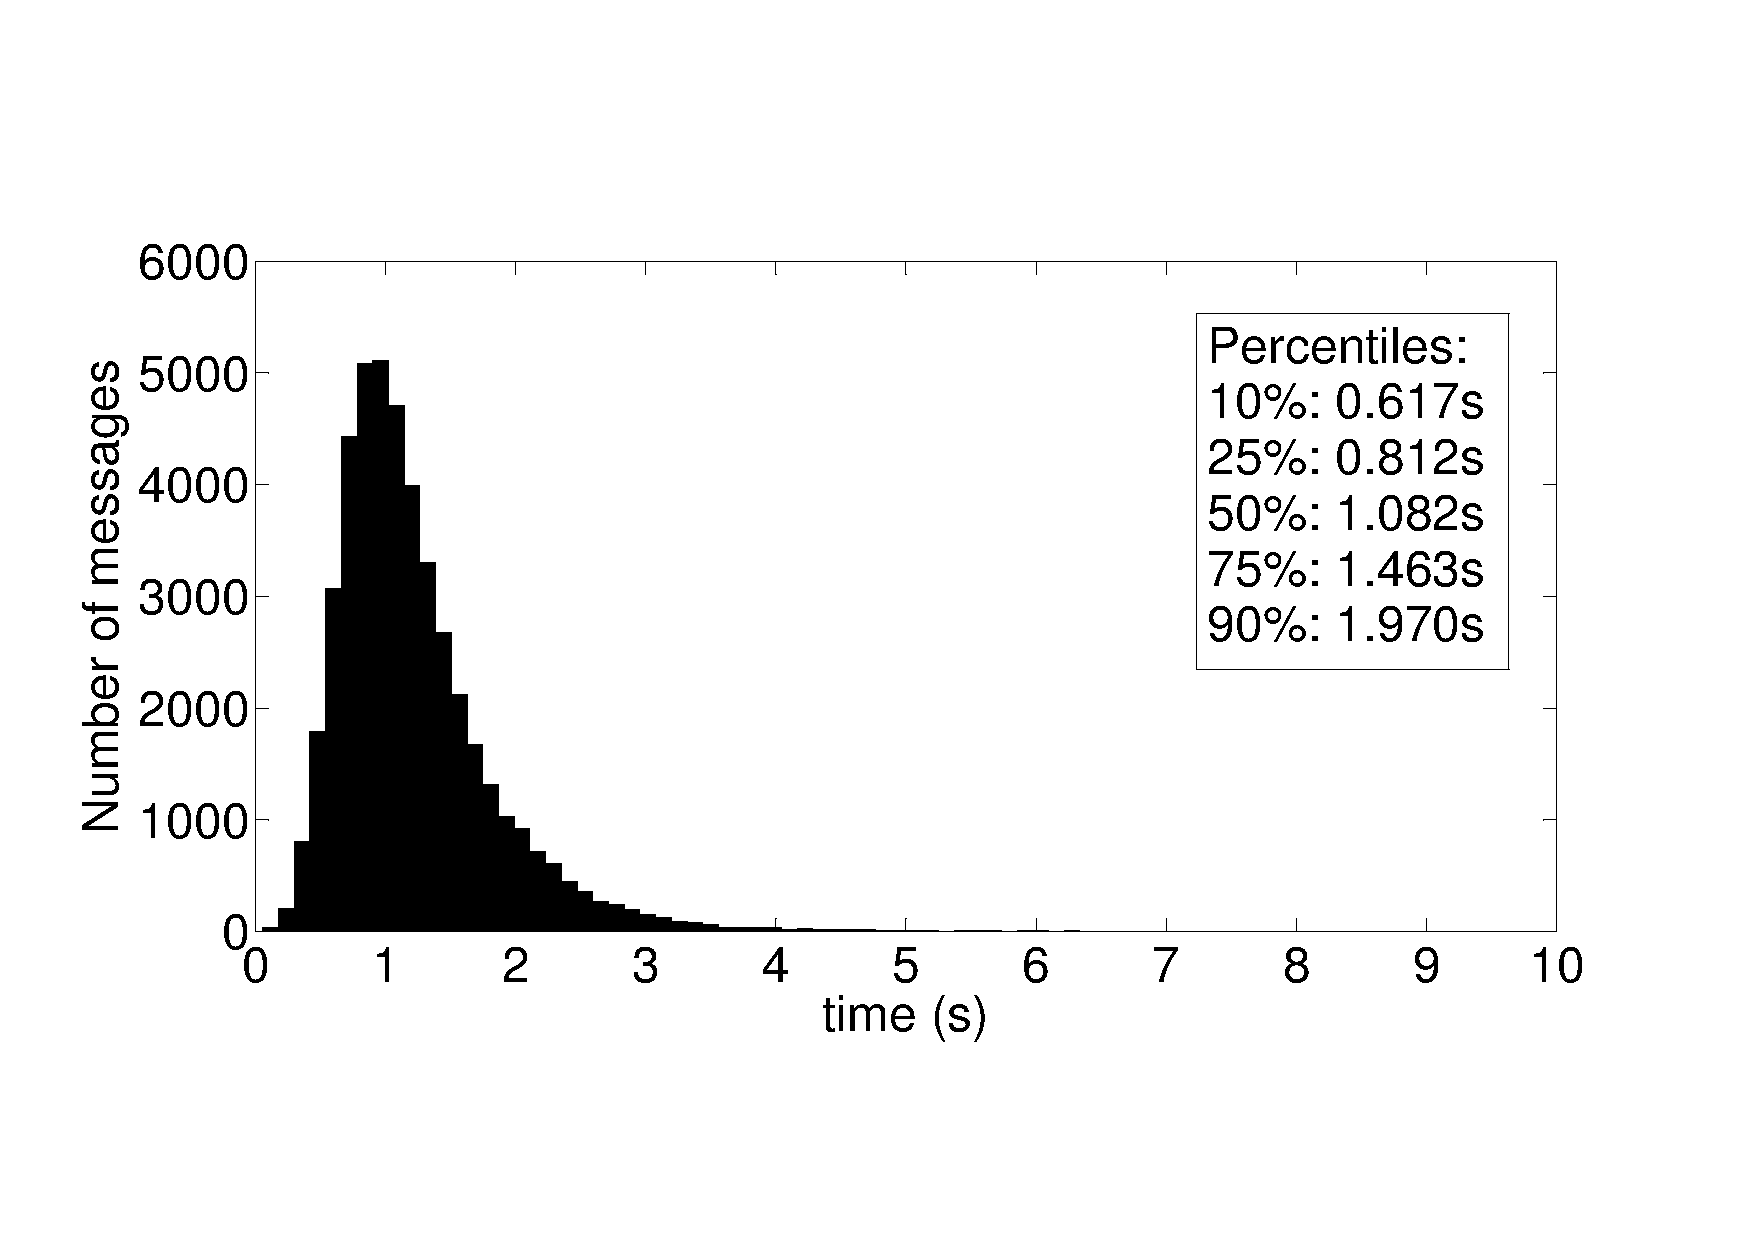
\includegraphics[clip=true, viewport=5mm 65mm 265mm 205mm, width=\columnwidth]{overlay_put_sf}
 \caption{Overlay storage responsiveness}
 \label{fig_overlay_put_sf}
\end{figure}
%
Figure \ref{fig_overlay_put_sf} shows that to store an object in the overlay can take anywhere from 0.1 to 4 seconds.

\begin{figure}[htbp]
 \centering
 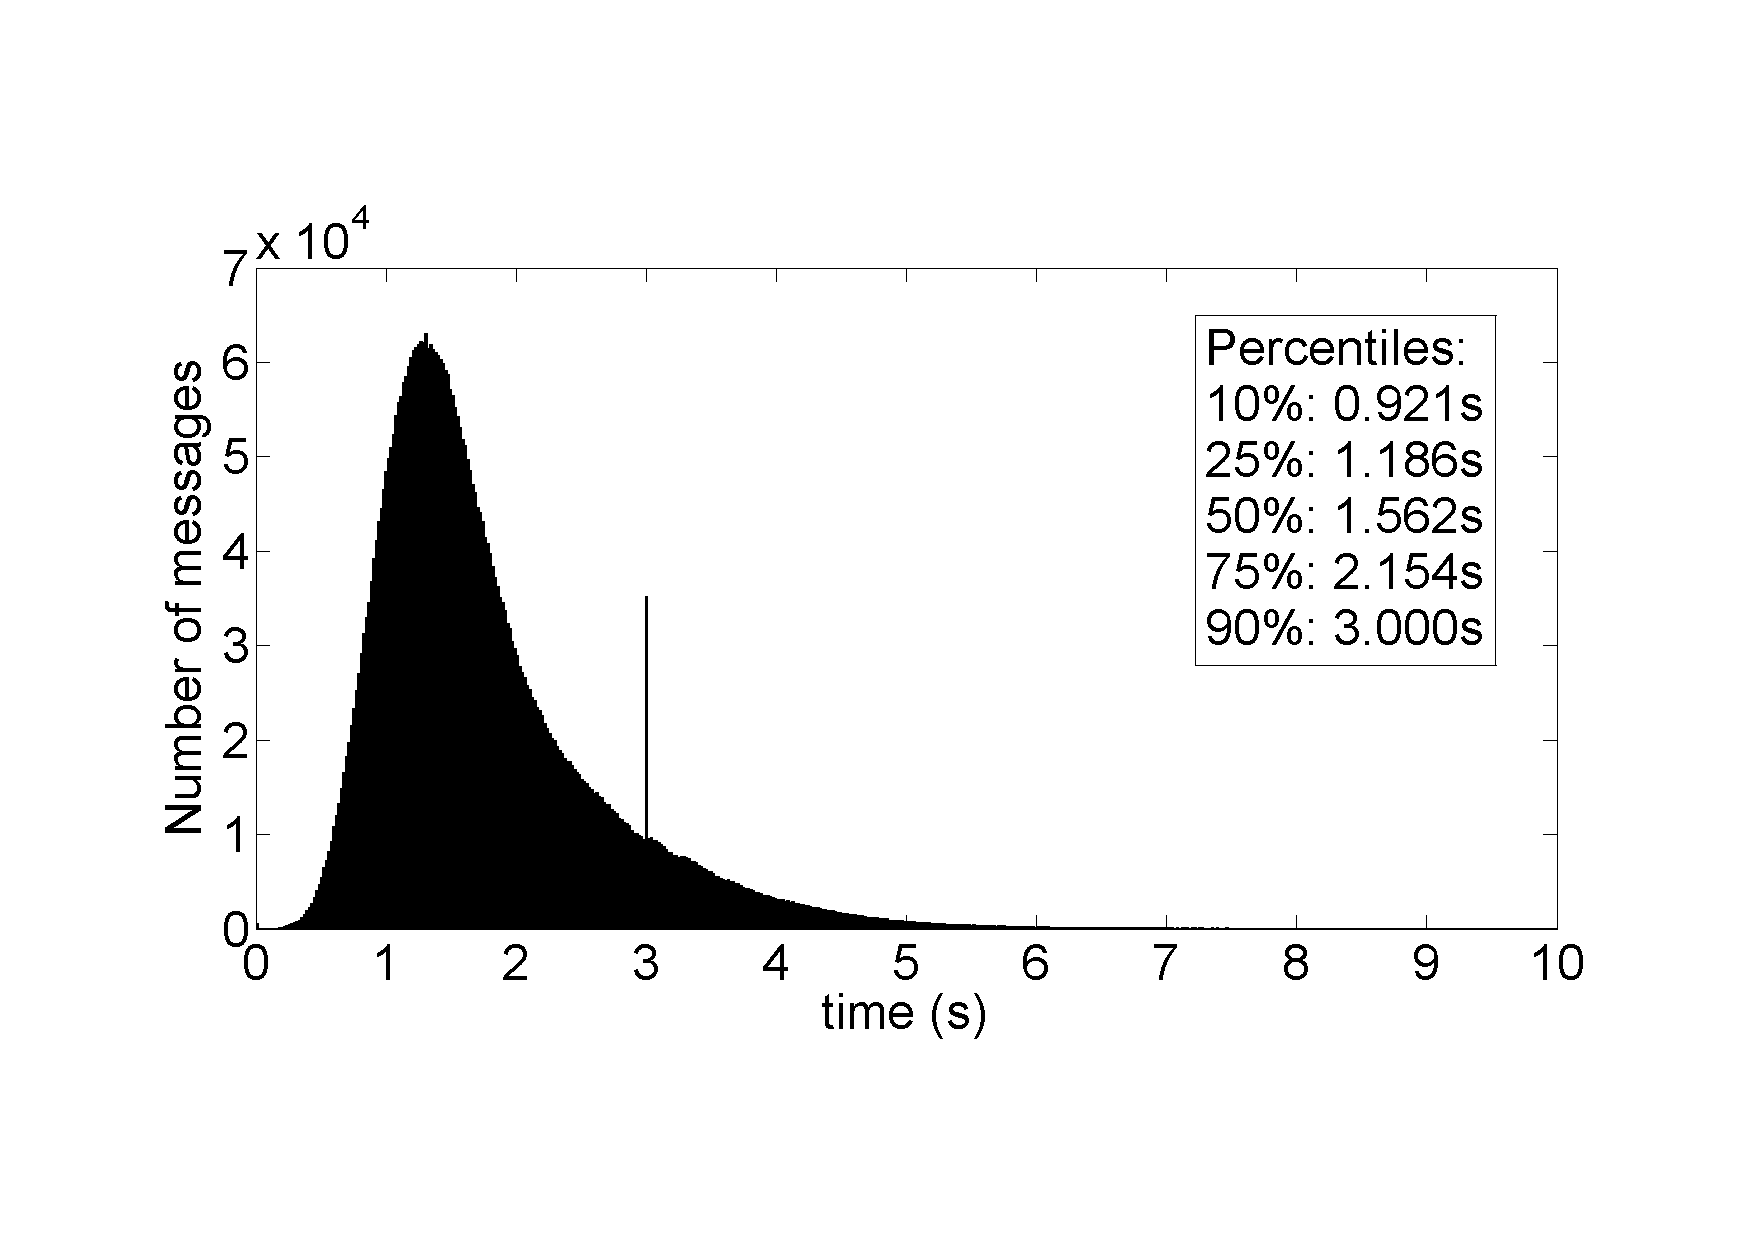
\includegraphics[clip=true, viewport=20mm 30mm 270mm 190mm, width=\columnwidth]{overlay_get_sf}
 \caption{Overlay retrieval responsiveness}
 \label{fig_overlay_get_sf}
\end{figure}
%
Figure \ref{fig_overlay_get_sf} shows that to retrieve an object from the overlay can take anywhere from 0.1 to 6 seconds. Figure \ref{fig_overlay_get_sf} also shows a spike at 3 seconds, when overlay retrieval is performed. This means that a large number of requests take 3 seconds to complete. This is thought to be an artifact of Chord lookup performance due to timeouts as set up in the Oversim simulation.

Overlay storage and retrieval has a high standard deviation when compared to group storage and retrieval as will be shown in the next sections.


\subsection{Group storage}

\subsubsection{Fast storage and fast or parallel retrieval}
\label{group_put_f_fp}

Figure \ref{fig_group_put_fp} shows the distribution of group storage for fast storage and fast or parallel retrieval. During simulation it was found that the storage responsiveness distribution is not influenced by the retrieval distribution. Likewise, the retrieval responsiveness distribution is not influenced by the storage types as will be shown later in this section.

\begin{figure}[htbp]
 \centering
 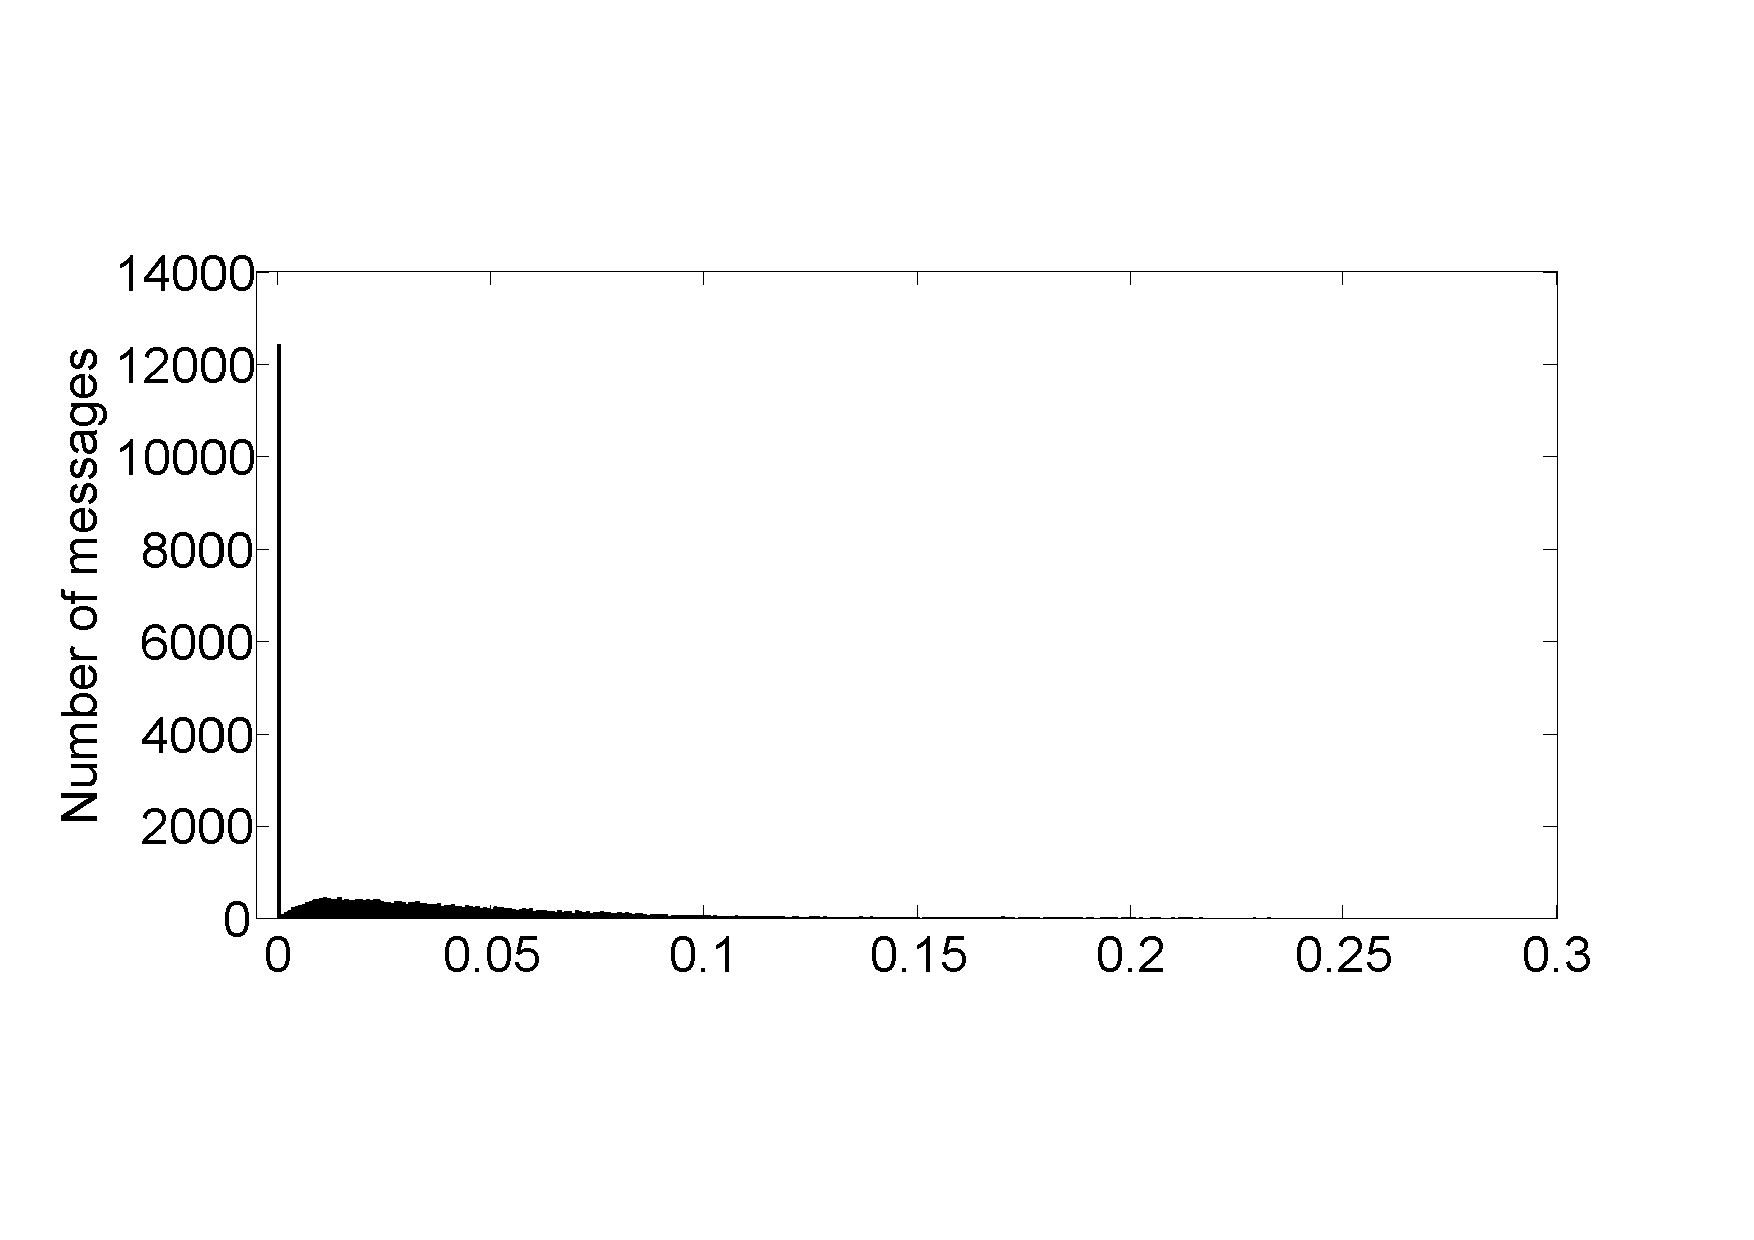
\includegraphics[clip=true, viewport=10mm 30mm 270mm 185mm, width=\columnwidth]{group_put_fp}
 \caption{Group storage responsiveness for fast storage and fast or parallel retrieval}
 \label{fig_group_put_fp}
\end{figure}
%
Figure \ref{fig_group_put_fp} shows a high peak at close to zero seconds. This peak shows that a large number of storage requests have a small time compared to the rest of requests. These requests are the requests where the node generating the object is chosen to store the object. If the required number of replicas is high, compared to the group size, there is a high likelihood that the node originating the request will be chosen as a host node to the object. This is why there is such a large spike at close to zero.

Apart from the spike, Figure \ref{fig_group_put_fp} also shows that the responsiveness is distributed over a small range: from zero to 0.1 seconds.

\subsubsection{Safe storage and fast or parallel retrieval}
\begin{figure}[htbp]
 \centering
 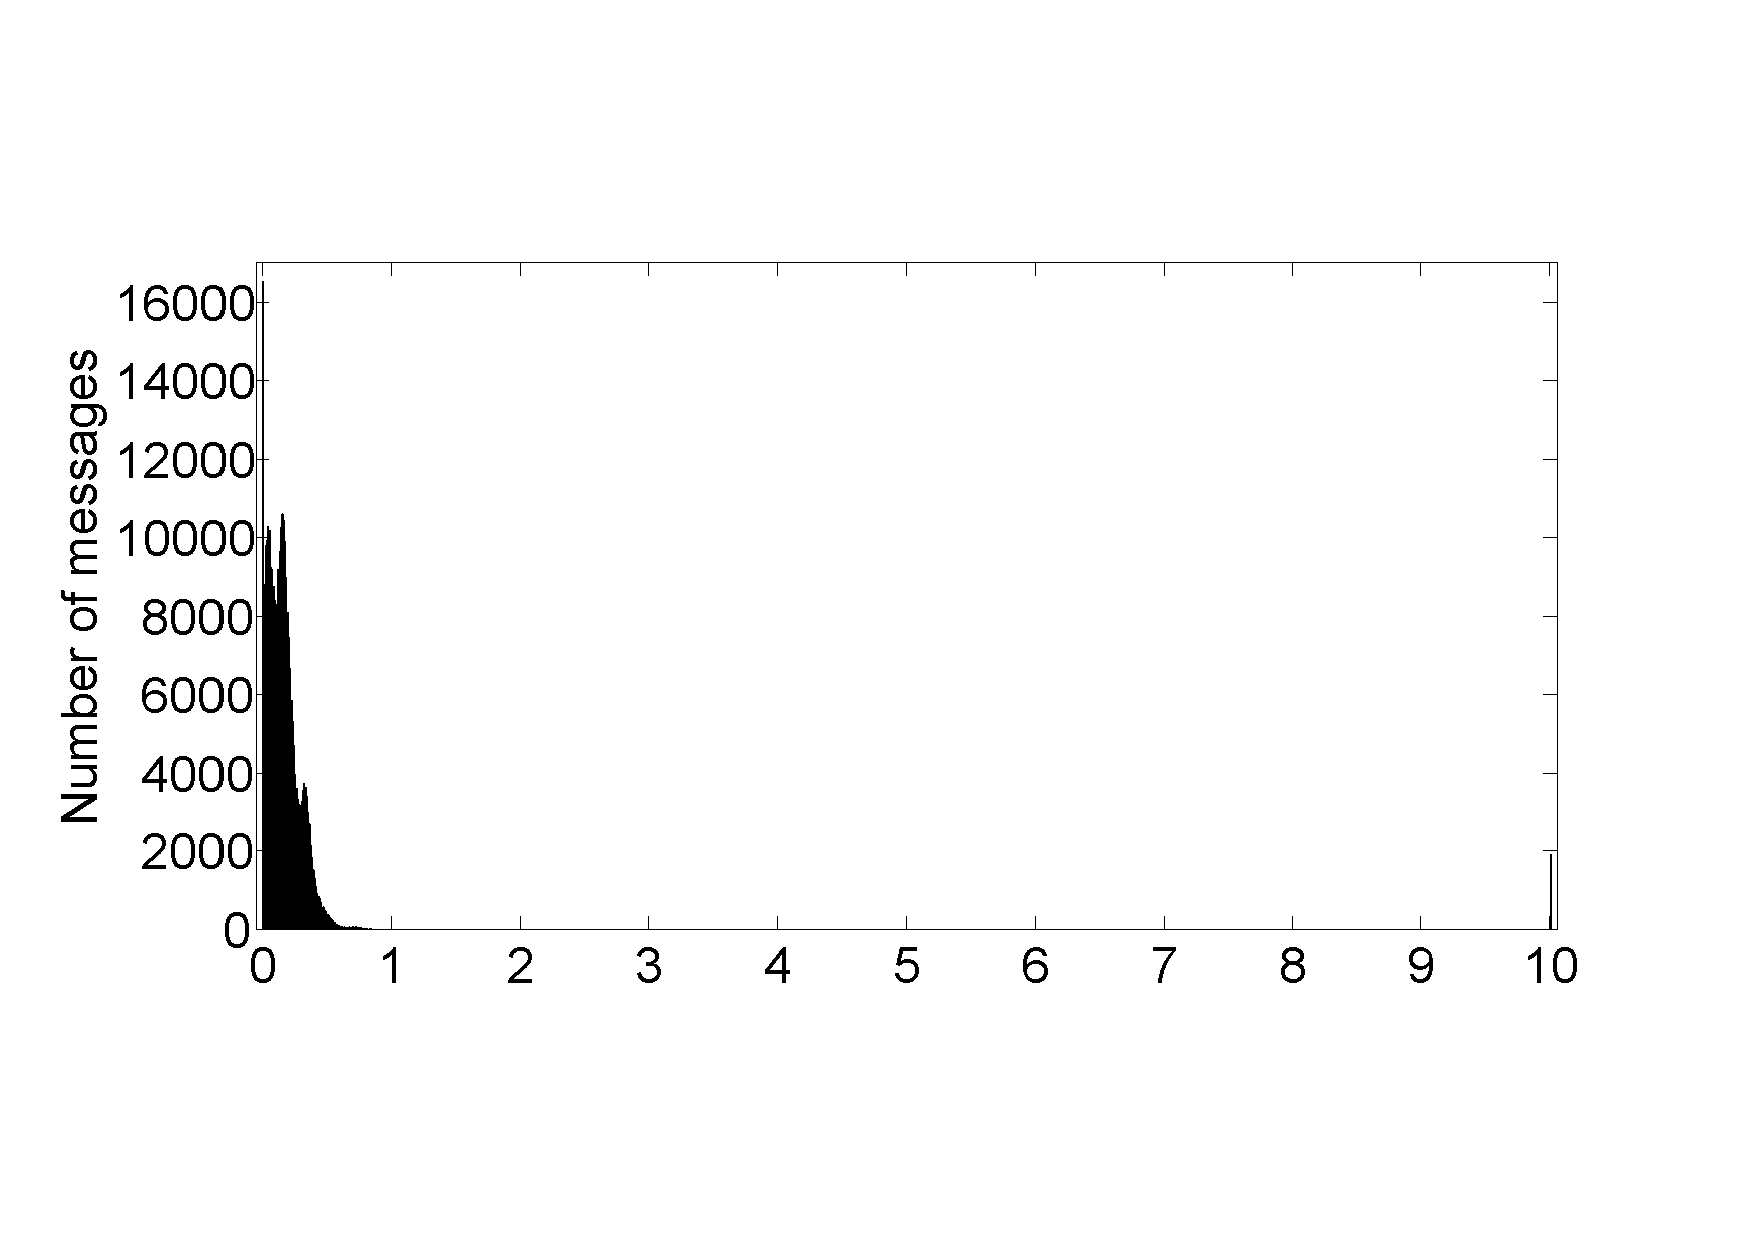
\includegraphics[clip=true, viewport=10mm 30mm 270mm 180mm, width=\columnwidth]{group_put_sf}
 \caption{Group storage responsiveness for safe storage and fast or parallel retrieval}
 \label{fig_group_put_sf}
\end{figure}
%
Figure \ref{fig_group_put_sf} shows the responsiveness distribution for safe storage and fast or parallel retrieval. Because safe storage is slower than fast storage, the mean responsiveness time is more. The maximum and minimum responsiveness values are also greater than for fast storage: from zero to 0.8 seconds. This is still smaller than the range of overlay storage values.

Figure \ref{fig_group_put_sf} also contains a spike at 10s. This is due to the storage timeout being set to 10s. What should be noted is that these responsiveness graphs shows both success and failure responsiveness. In other words, it shows how quickly a response is received, even if that response is a failure. The responses received from 10 s will all be failures, where no response was received from the destination node and an internal timeout occurred.

The ``bumps'' in Figure \ref{fig_group_put_sf} are similar to the ones seen in group retrieval in Figure \ref{fig_group_get_zoom_sf} and are artifacts of Oversim's SimpleUnderlay network structure, as discussed in Section \ref{lan_retrieval}. The large spike at zero seconds is also present for the same reason mentioned earlier.

\subsection{Group retrieval}
\subsubsection{Fast retrieval and safe or fast storage}
\begin{figure}[htbp]
 \centering
 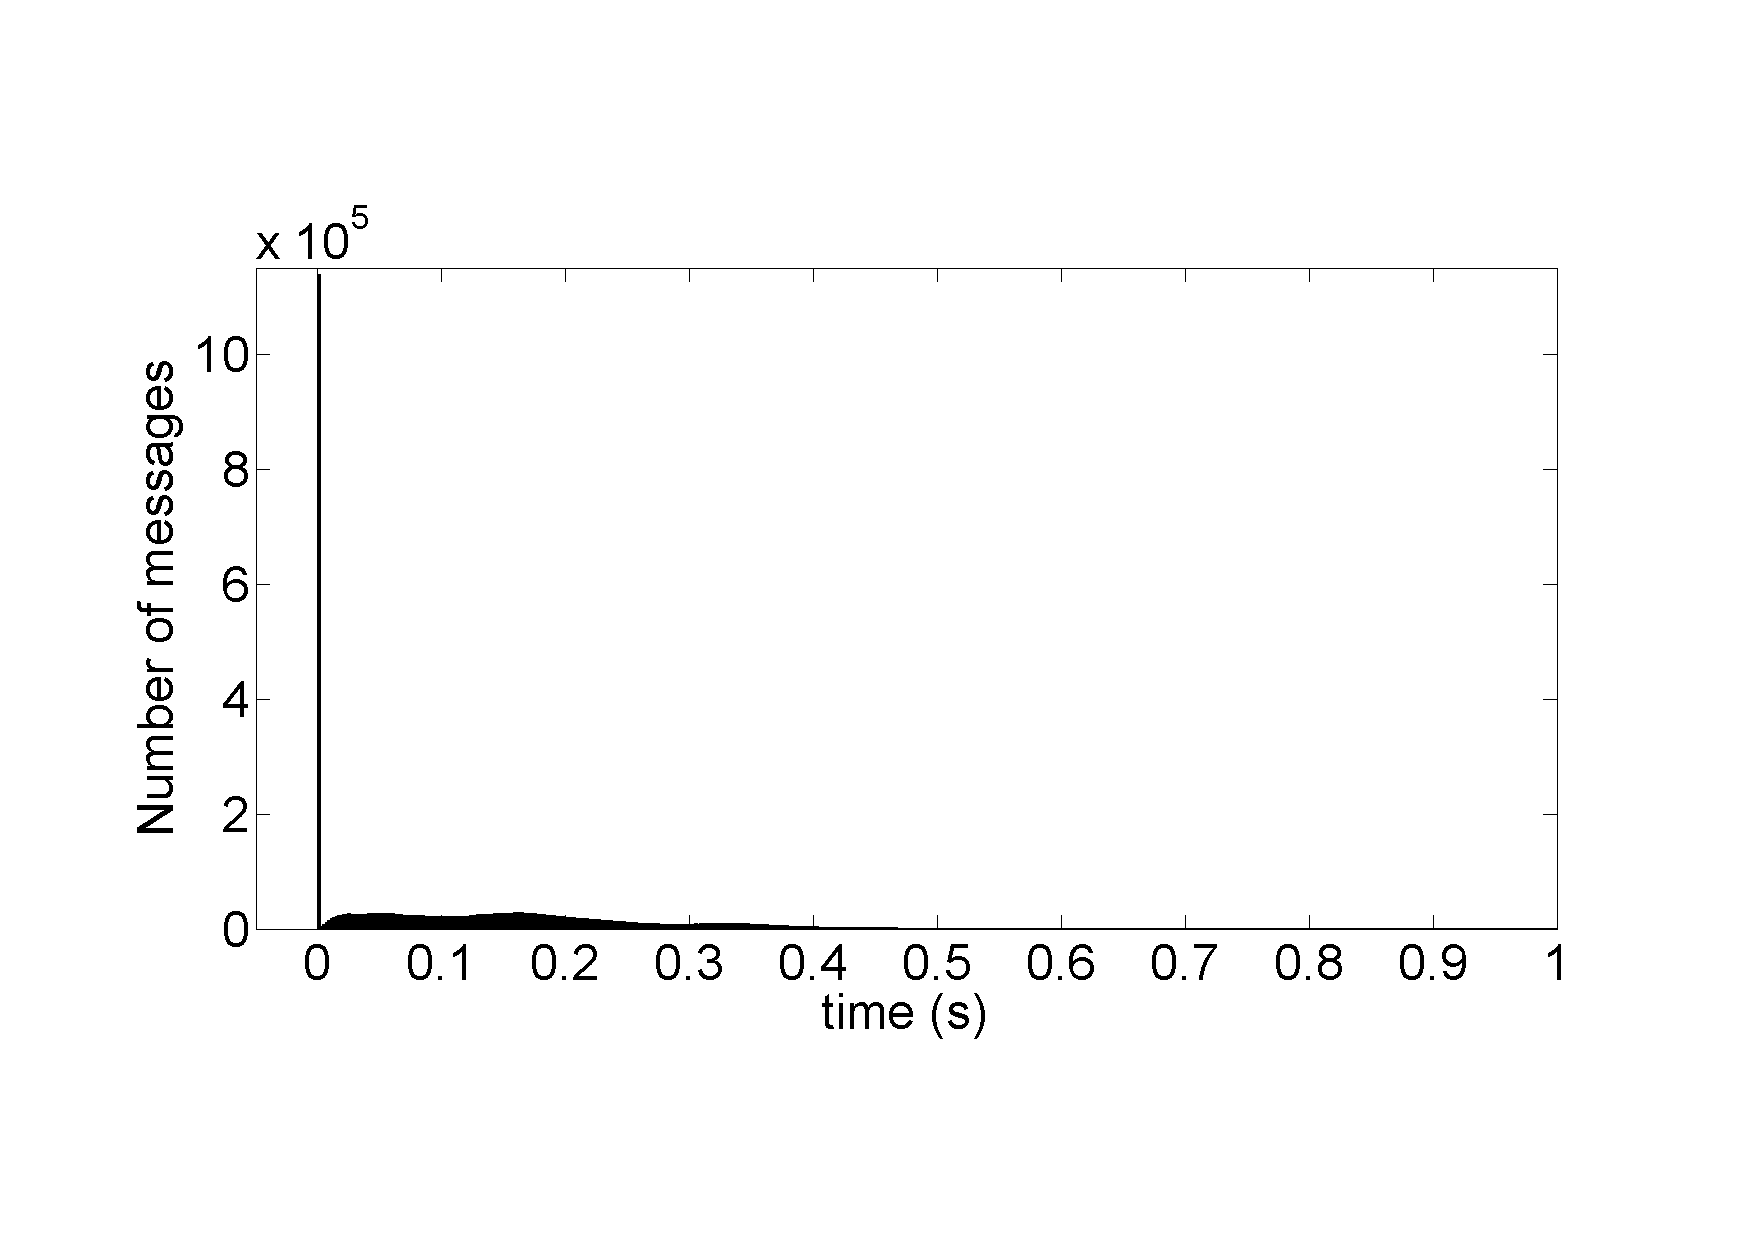
\includegraphics[clip=true, viewport=20mm 30mm 265mm 180mm, width=\columnwidth]{group_get_sf}
 \caption{Group retrieval responsiveness for safe or fast storage and fast retrieval}
 \label{fig_group_get_sf}
\end{figure}
%
Figure \ref{fig_group_get_sf} shows group retrieval responsiveness for fast retrieval and safe or fast storage. This type of retrieval also shows a spike at zero seconds due to nodes requesting objects from the network and those objects being found in the locally stored root object store. Because of the high number of replicas compared to the average group size used in the simulation, many of the requests can be locally served, which greatly increases responsiveness.

\begin{figure}[htbp]
 \centering
 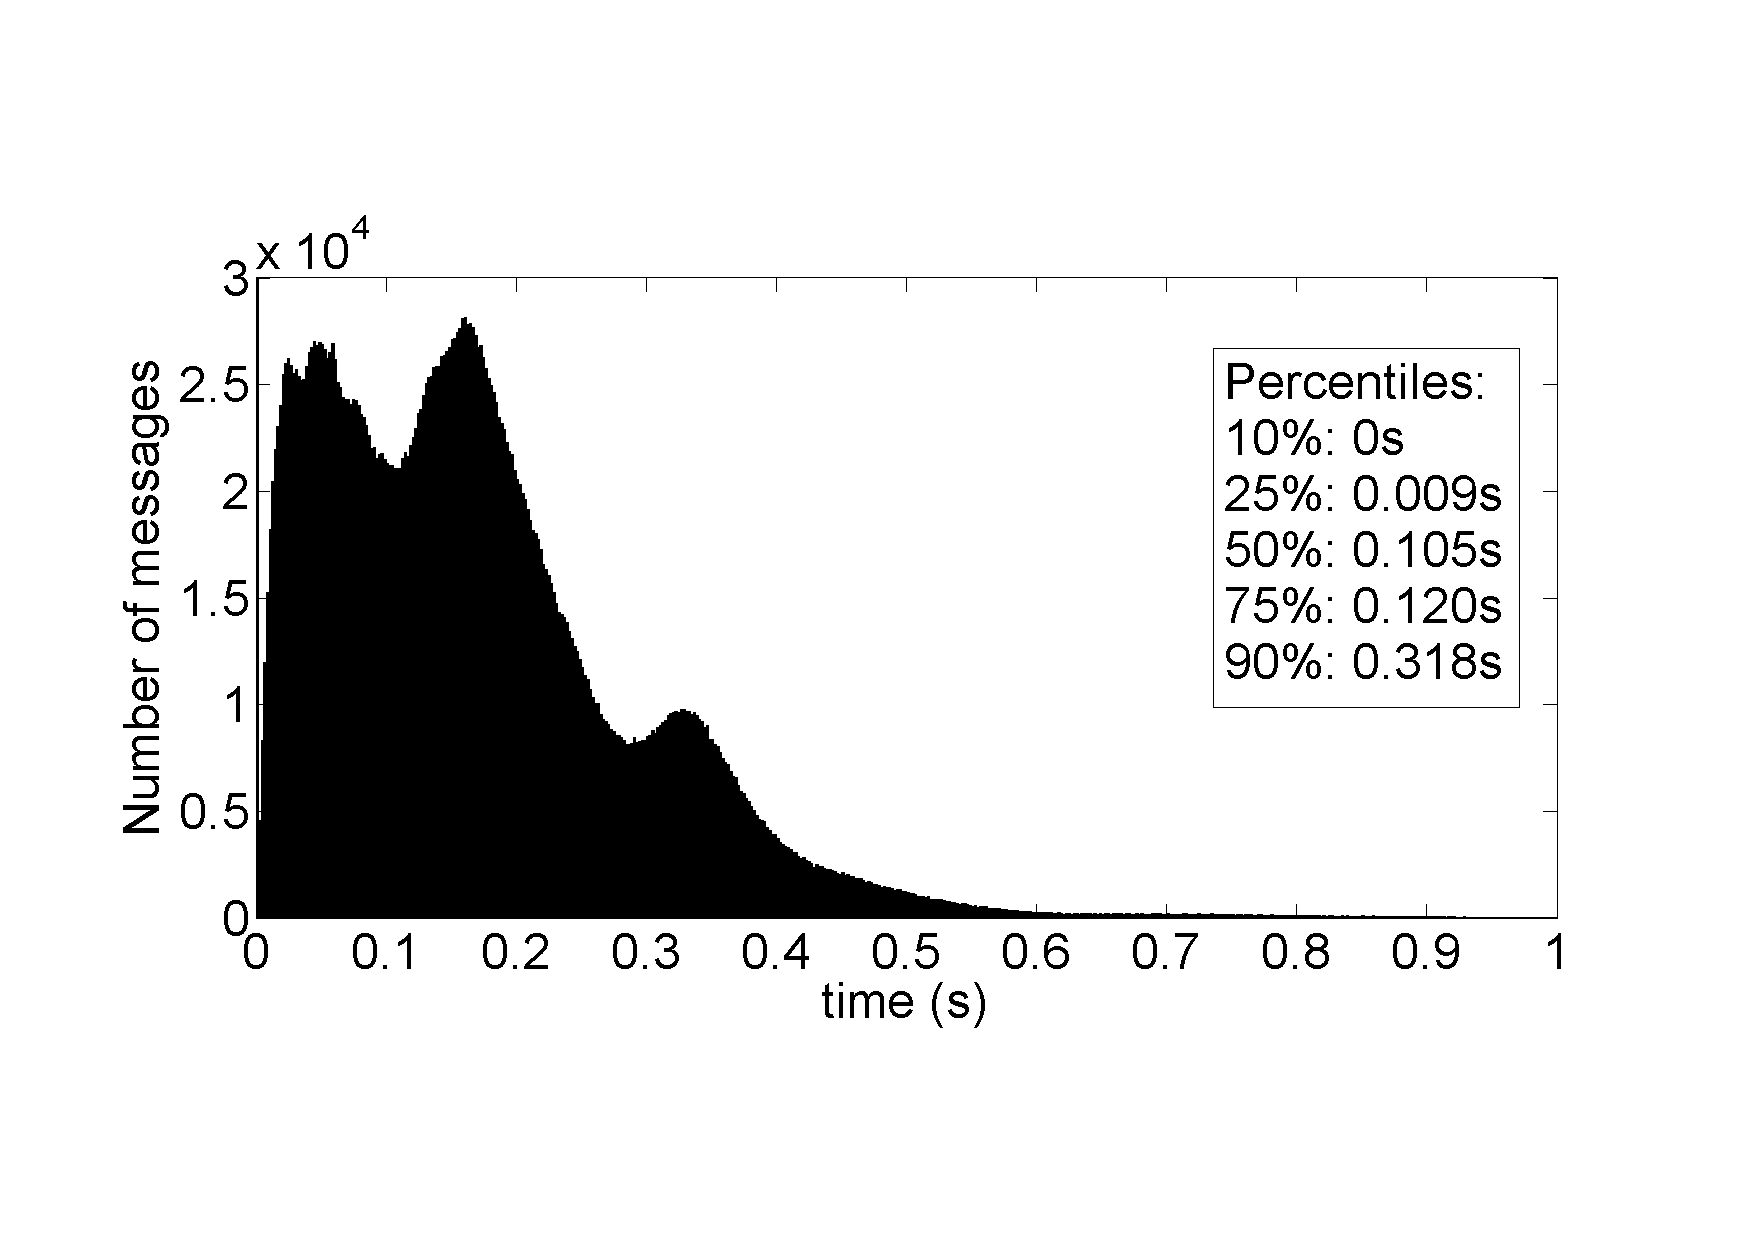
\includegraphics[clip=true, viewport=20mm 30mm 265mm 180mm, width=\columnwidth]{group_get_zoom_sf}
 \caption{Enlarged view of the group retrieval responsiveness for safe or fast storage and fast retrieval}
 \label{fig_group_get_zoom_sf}
\end{figure}
%
The details of Figure \ref{fig_group_get_sf} can clearly be seen in Figure \ref{fig_group_get_zoom_sf}, which presents an enlarged view of Figure \ref{fig_group_get_sf}. This figure also shows the multiple ``bumps'', which is an artifact of the underlying physical layer, as described in Section \ref{lan_retrieval}. The figure shows that fast group retrieval responsiveness varies from zero to 0.9 seconds.

\subsubsection{Parallel retrieval and safe or fast storage}
\begin{figure}[htbp]
 \centering
 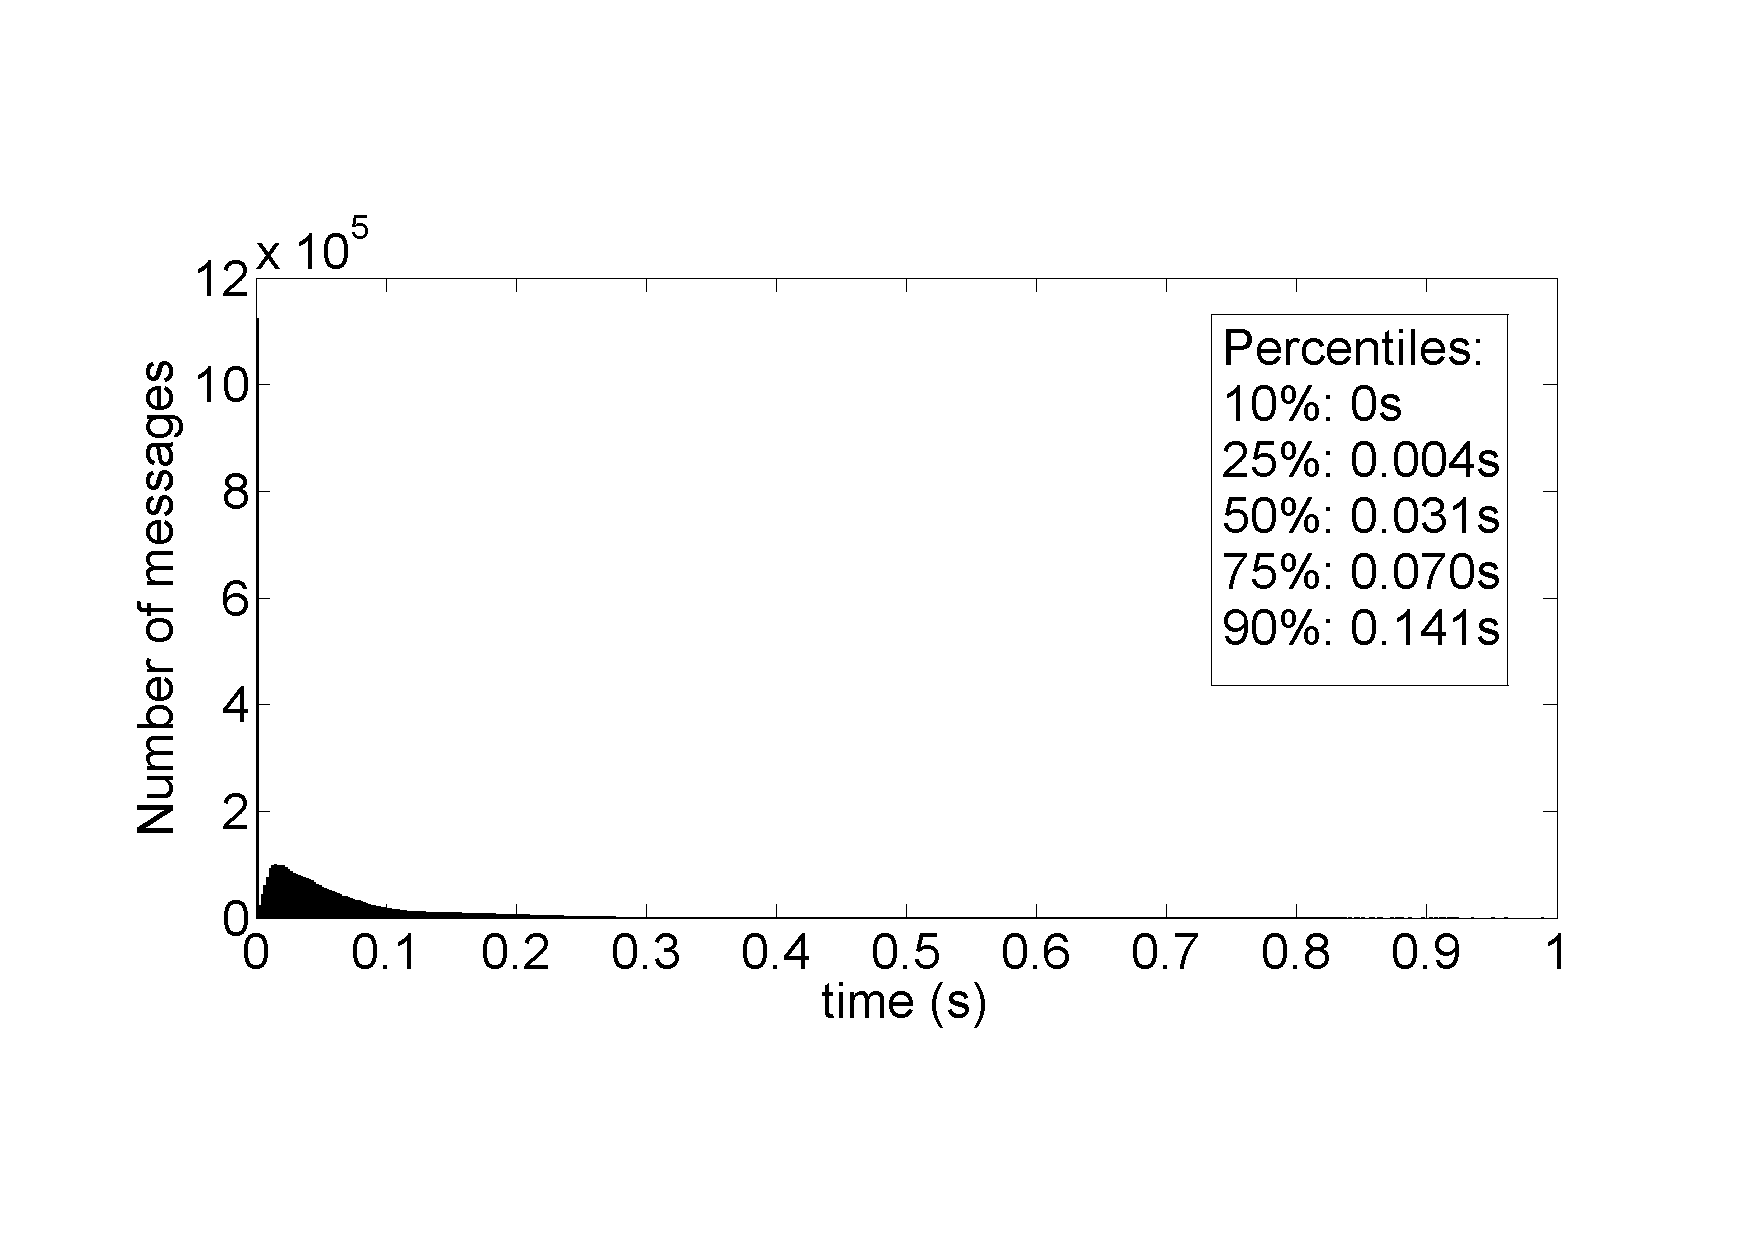
\includegraphics[clip=true, viewport=20mm 30mm 265mm 180mm, width=\columnwidth]{group_get_fp}
 \caption{Group retrieval responsiveness for safe or fast storage and parallel retrieval}
 \label{fig_group_get_fp}
\end{figure}

\begin{figure}[htbp]
 \centering
 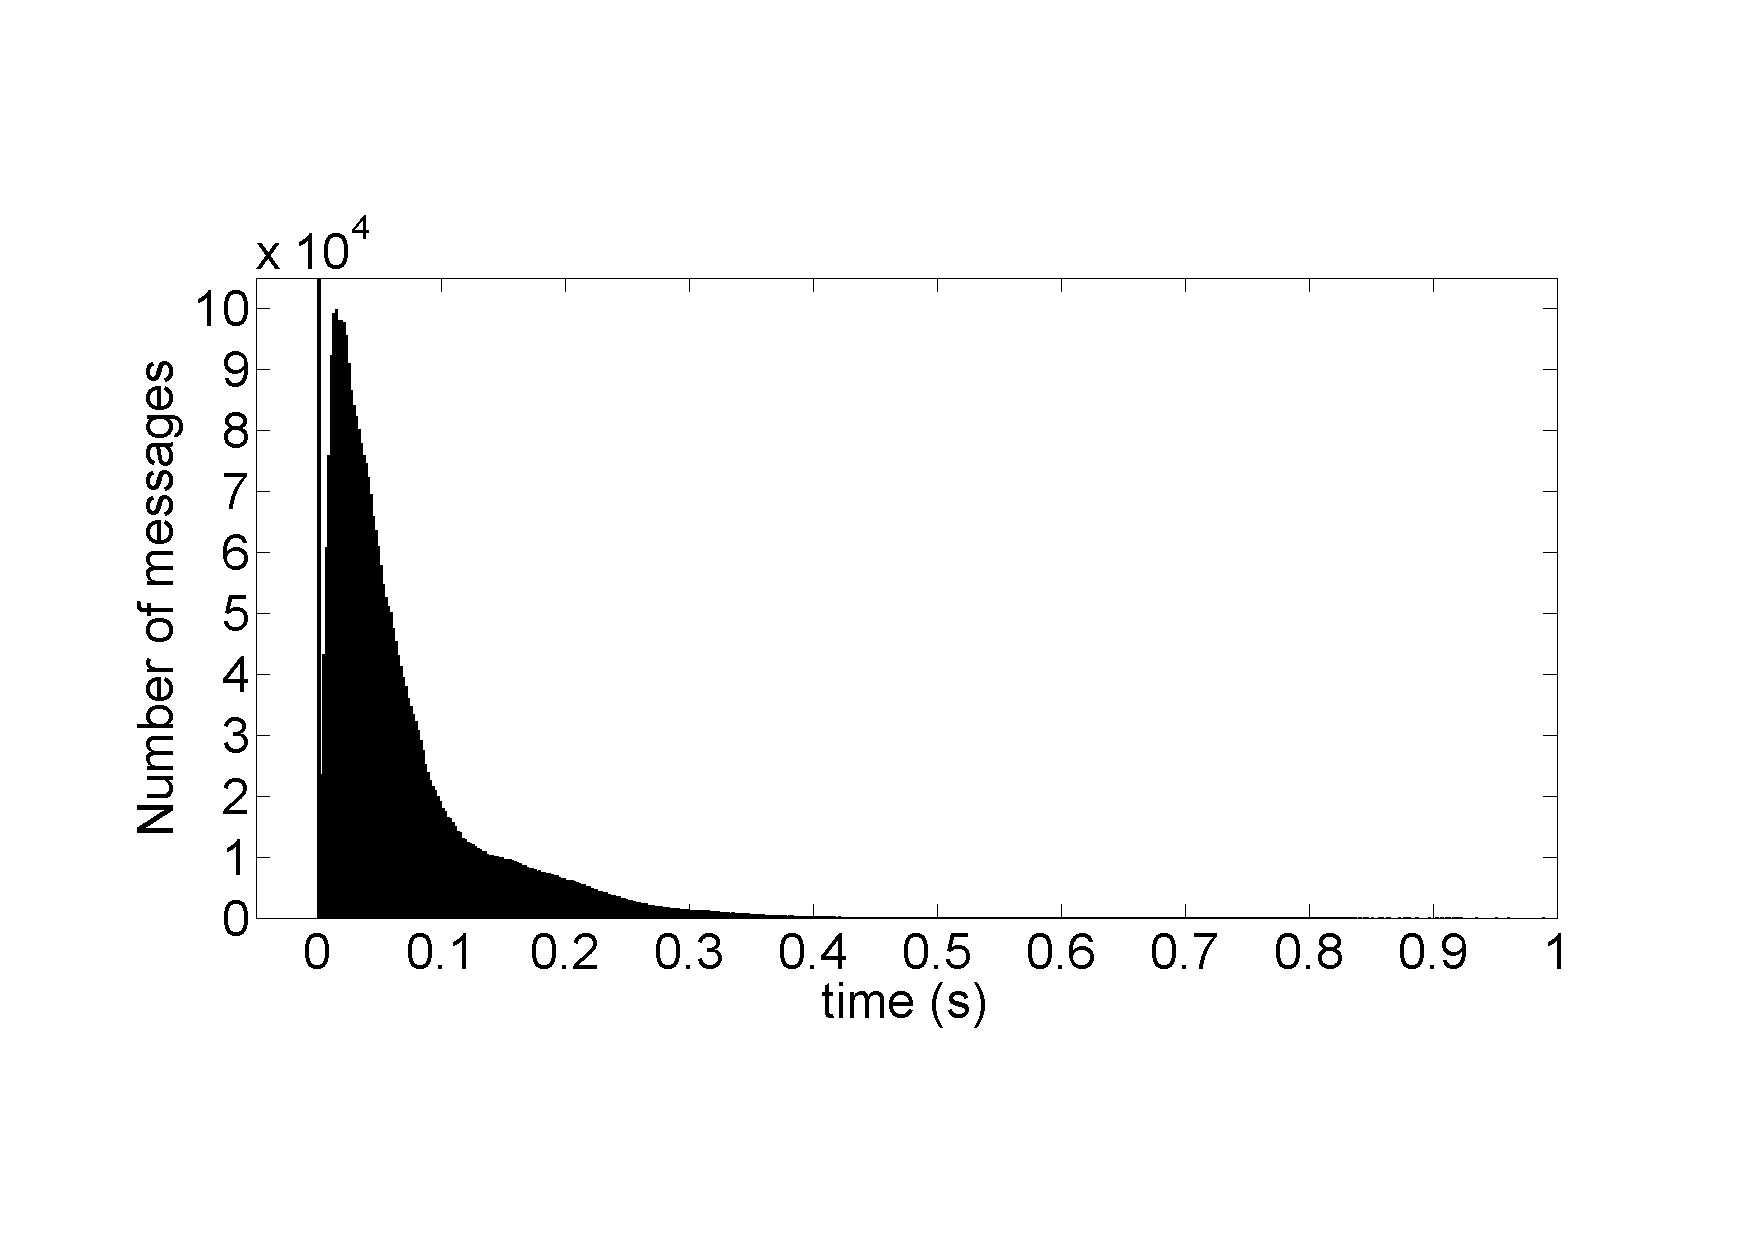
\includegraphics[clip=true, viewport=20mm 30mm 265mm 180mm, width=\columnwidth]{group_get_zoom_fp}
 \caption{Enlarged view of the group retrieval responsiveness for safe or fast storage and parallel retrieval}
 \label{fig_group_get_zoom_fp}
\end{figure}
%
Figure \ref{fig_group_get_fp} shows group retrieval responsiveness for parallel retrieval and fast or safe storage and Figure \ref{fig_group_get_zoom_fp} shows the enlarged view. Apart from the higher responsiveness, explained in Section \ref{pithos_resp_rel_results}, parallel retrieval also has a smaller range of values: from zero to 0.4 seconds.

The shape of Figure \ref{fig_group_get_zoom_fp} differs from that of Figure \ref{fig_group_get_zoom_sf} due to the difference between selecting a single random node ($1/r$) in the group for retrieval, to selecting the fastest of $r$ nodes in the group for retrieval, where $r$ is the number of object replicas currently in the group.

\subsection{LAN performance}
\label{lan_retrieval}

Figures \ref{fig_group_put_sf} and \ref{fig_group_get_zoom_sf} show ``bumps'' that were described as being underlying network artifacts. To show that this, another simulation run is performed where the coordinate-based system used in Oversim is replaced by all links being set to have 1ms latency and jitter of 0.1\%. The purpose of this is to show that group storage has the correct expected number of hops, that the ``bumps'' are not inherent to Pithos and that Pithos's performance is greatly improved when the underlaying network architecture has improved performance.

\begin{figure}[htbp]
 \centering
 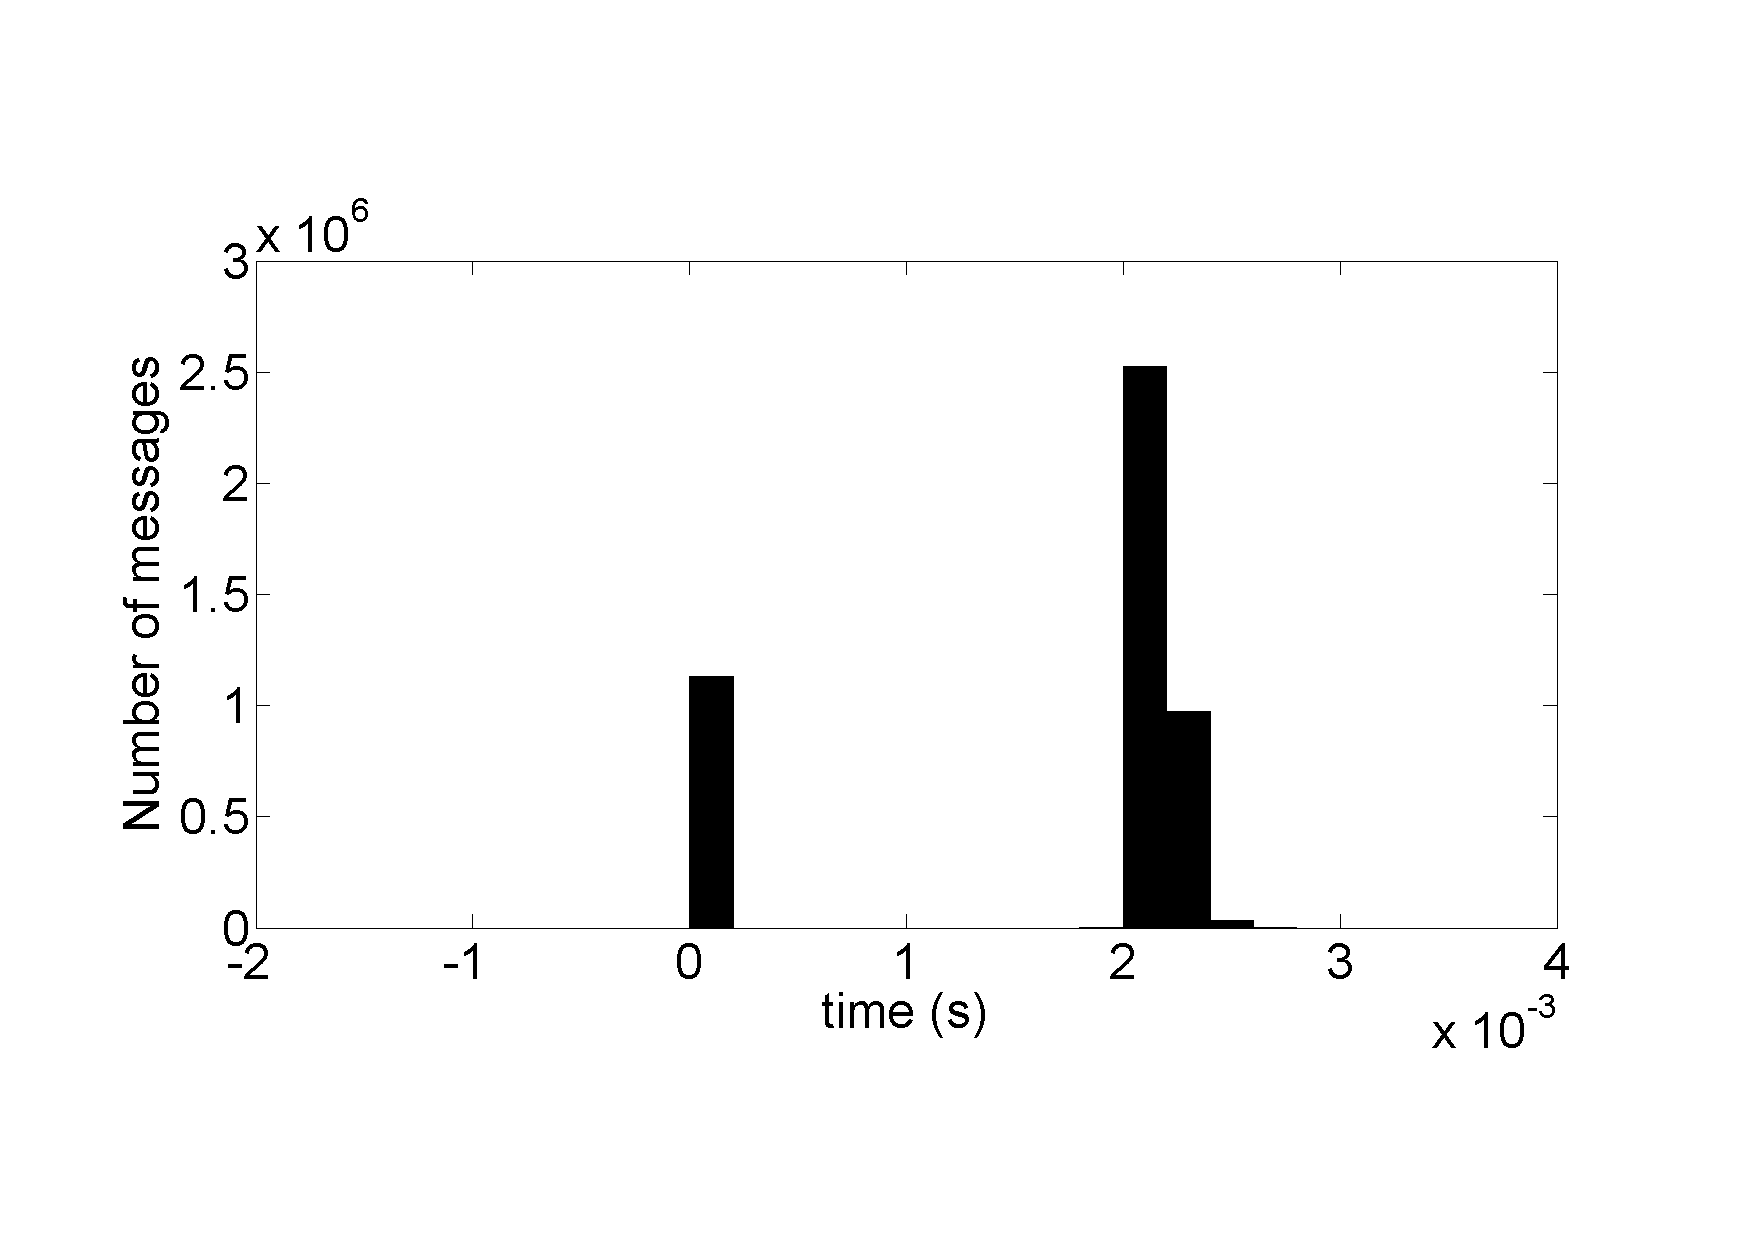
\includegraphics[clip=true, viewport=20mm 30mm 265mm 180mm, width=\columnwidth]{group_get_lan}
 \caption{Group retrieval responsiveness for fast storage and fast retrieval, running on a 1ms underlay network.}
 \label{fig_group_get_lan}
\end{figure}
%
Figure \ref{fig_group_get_lan} shows group retrieval performance for fast storage and fast retrieval, running on a 1ms underlay network. This figure shows the same operation shown in Figure \ref{fig_group_get_zoom_sf}, but for the underlay being a fixed 1ms underlay, instead of a coordinate-based underlay.

Two main spikes are seen in the figure, one at 0s and another at 2ms. There are no other measured times. This is what is expected from group storage, since every request in group storage is zero hops or two hope. For two hops, one hop is required to sent the request, and another to receive the response, which gives $2\times 1 ms = 2 ms$. The zero hops case was explained in Section \ref{group_put_f_fp}.

No additional spikes are perceived, as opposed to the ``bumps'' seen earlier. The mean group storage performance has improved to 1.6ms, from the 192ms for the coordinate-based underlay network.

\subsection{Overall storage}

\subsubsection{Fast storage and fast or parallel retrieval}
After having presented the separate responsiveness profiles for overlay and group storage, the overall Pithos responsiveness is presented here which is a combination of the responsiveness profiles of the underlying group and overlay responsiveness.

\begin{figure}[htbp]
 \centering
 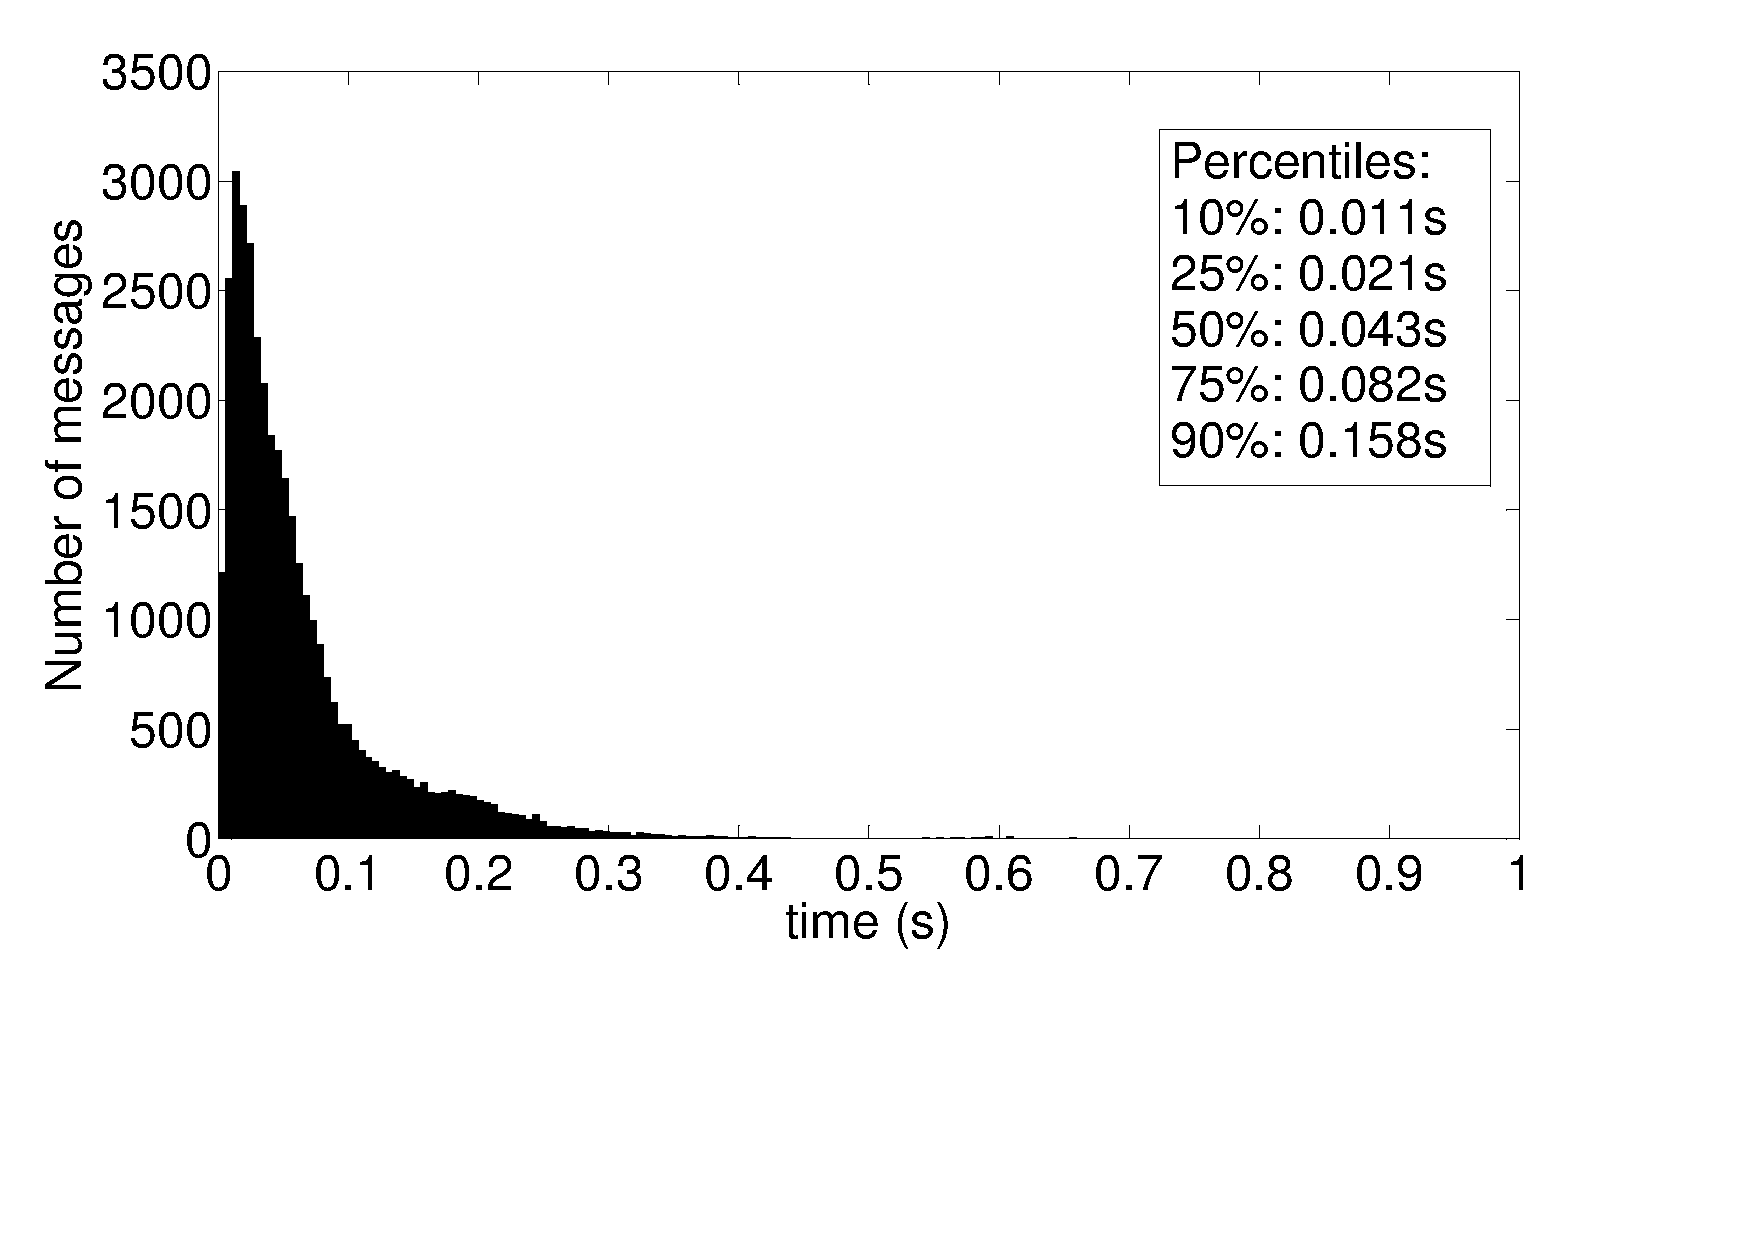
\includegraphics[clip=true, viewport=5mm 35mm 265mm 190mm, width=\columnwidth]{overall_put_ff}
 \caption{Overall storage responsiveness for fast storage and fast or parallel retrieval}
 \label{fig_overall_put_ff}
\end{figure}
%
Figure \ref{fig_overall_put_ff} shows the overall storage responsiveness for fast storage and fast or parallel retrieval. The shape is similar to that of Figure \ref{fig_group_get_zoom_fp}. A seemingly exponential distribution, due to the first successful storage response from group storage being sent to the higher layer. This has the effect of taking all responses and choosing the fastest one. Exactly the same mechanism as with parallel retrieval. Fast storage responsiveness ranges from zero to 0.3 seconds.

\subsubsection{Safe storage and fast or parallel retrieval}
\begin{figure}[htbp]
 \centering
 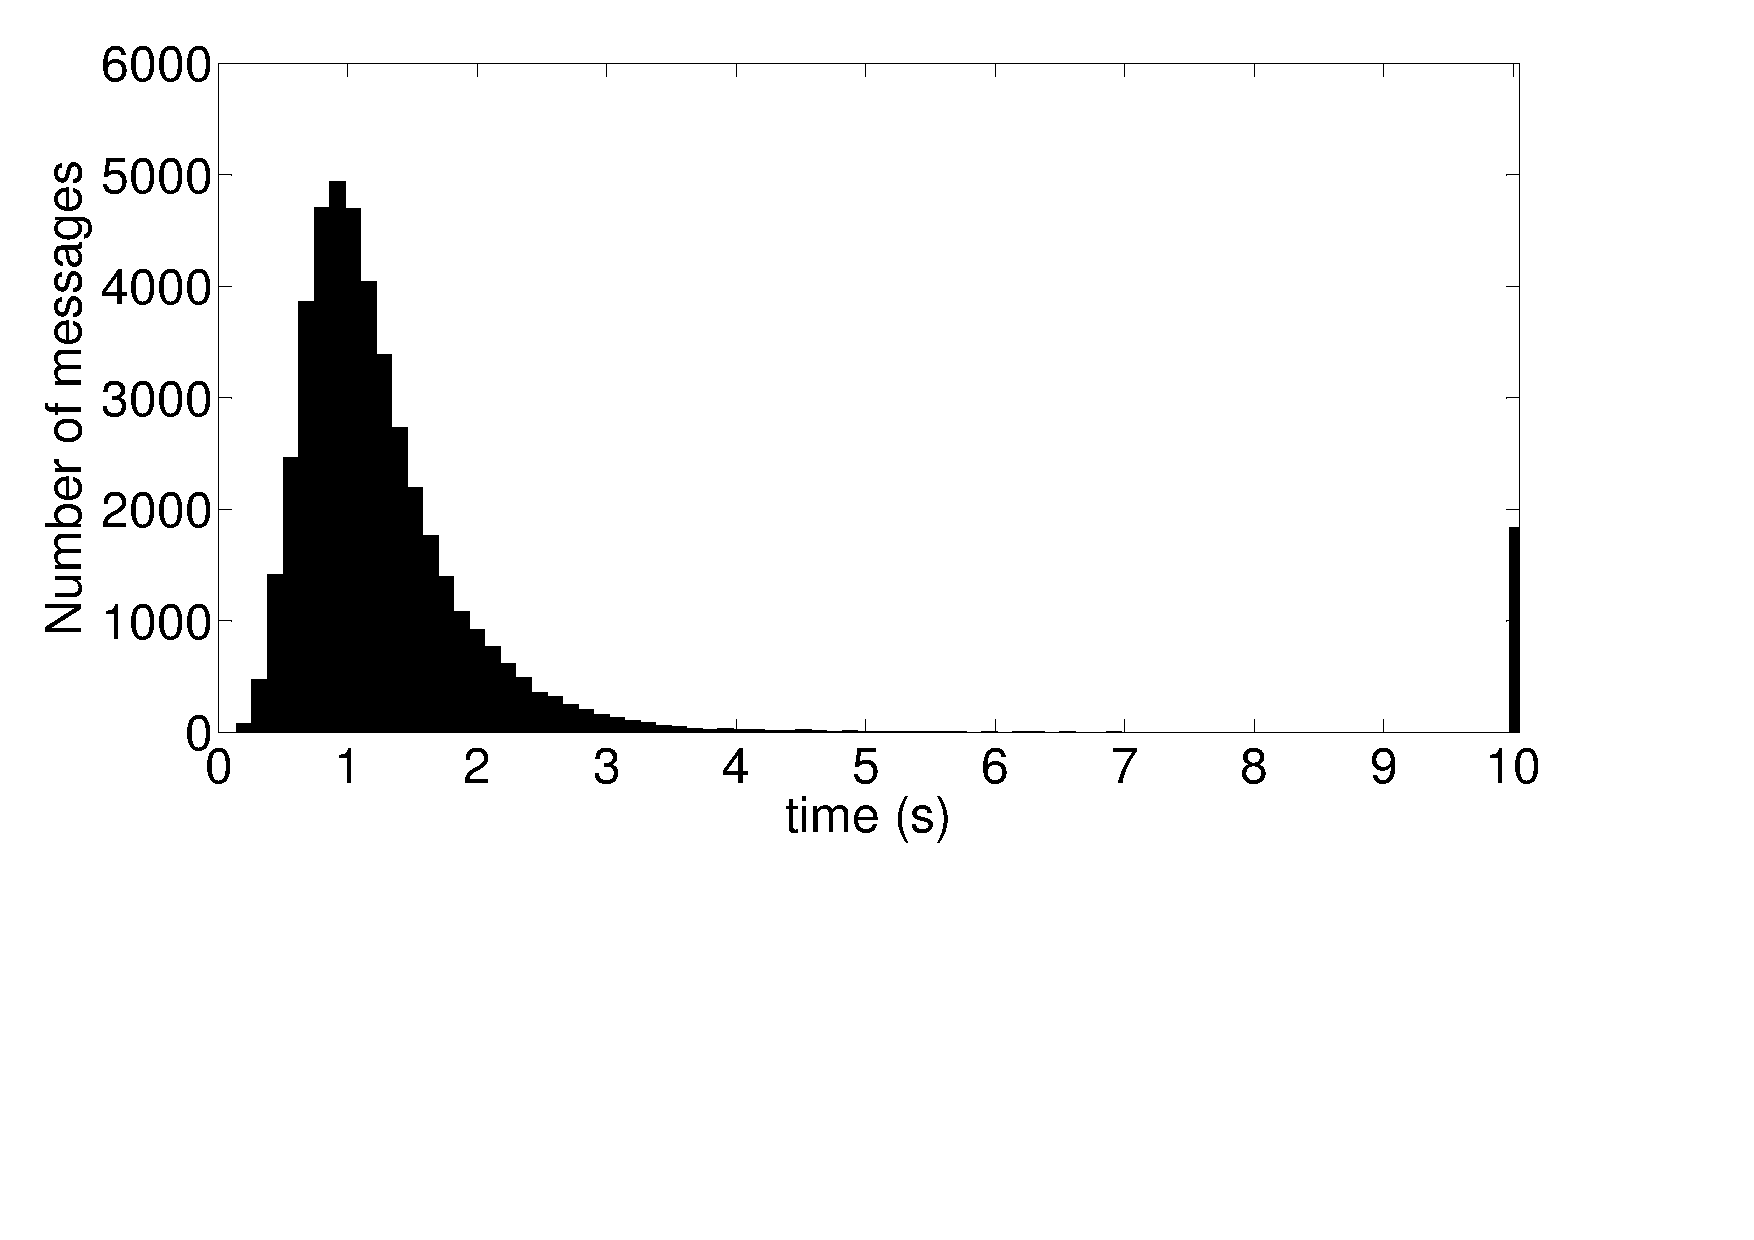
\includegraphics[clip=true, viewport=5mm 60mm 265mm 205mm, width=\columnwidth]{overall_put_sf}
 \caption{Overall storage responsiveness for safe storage and fast or parallel retrieval}
 \label{fig_overall_put_sf}
\end{figure}
%
Figure \ref{fig_overall_put_sf} shows the overall safe storage distribution for fast or parallel retrieval. Because a response is only sent from the group and overlay storage modules to the peer logic module when sufficiently many group responses have been received and when the overlay response has been received, the distribution takes on a shape exactly like the overlay storage distribution of Figure \ref{fig_overlay_put_sf}.

The reason why the shape has no correspondence to group storage responsiveness is because, as previously shown, overlay storage is always slower than group storage. Because safe storage always waits for the reply from the overlay storage module, it has the same shape and values as overlay storage.

\subsection{Overall retrieval}
\subsubsection{Fast retrieval and safe or fast storage}
\begin{figure}[htbp]
 \centering
 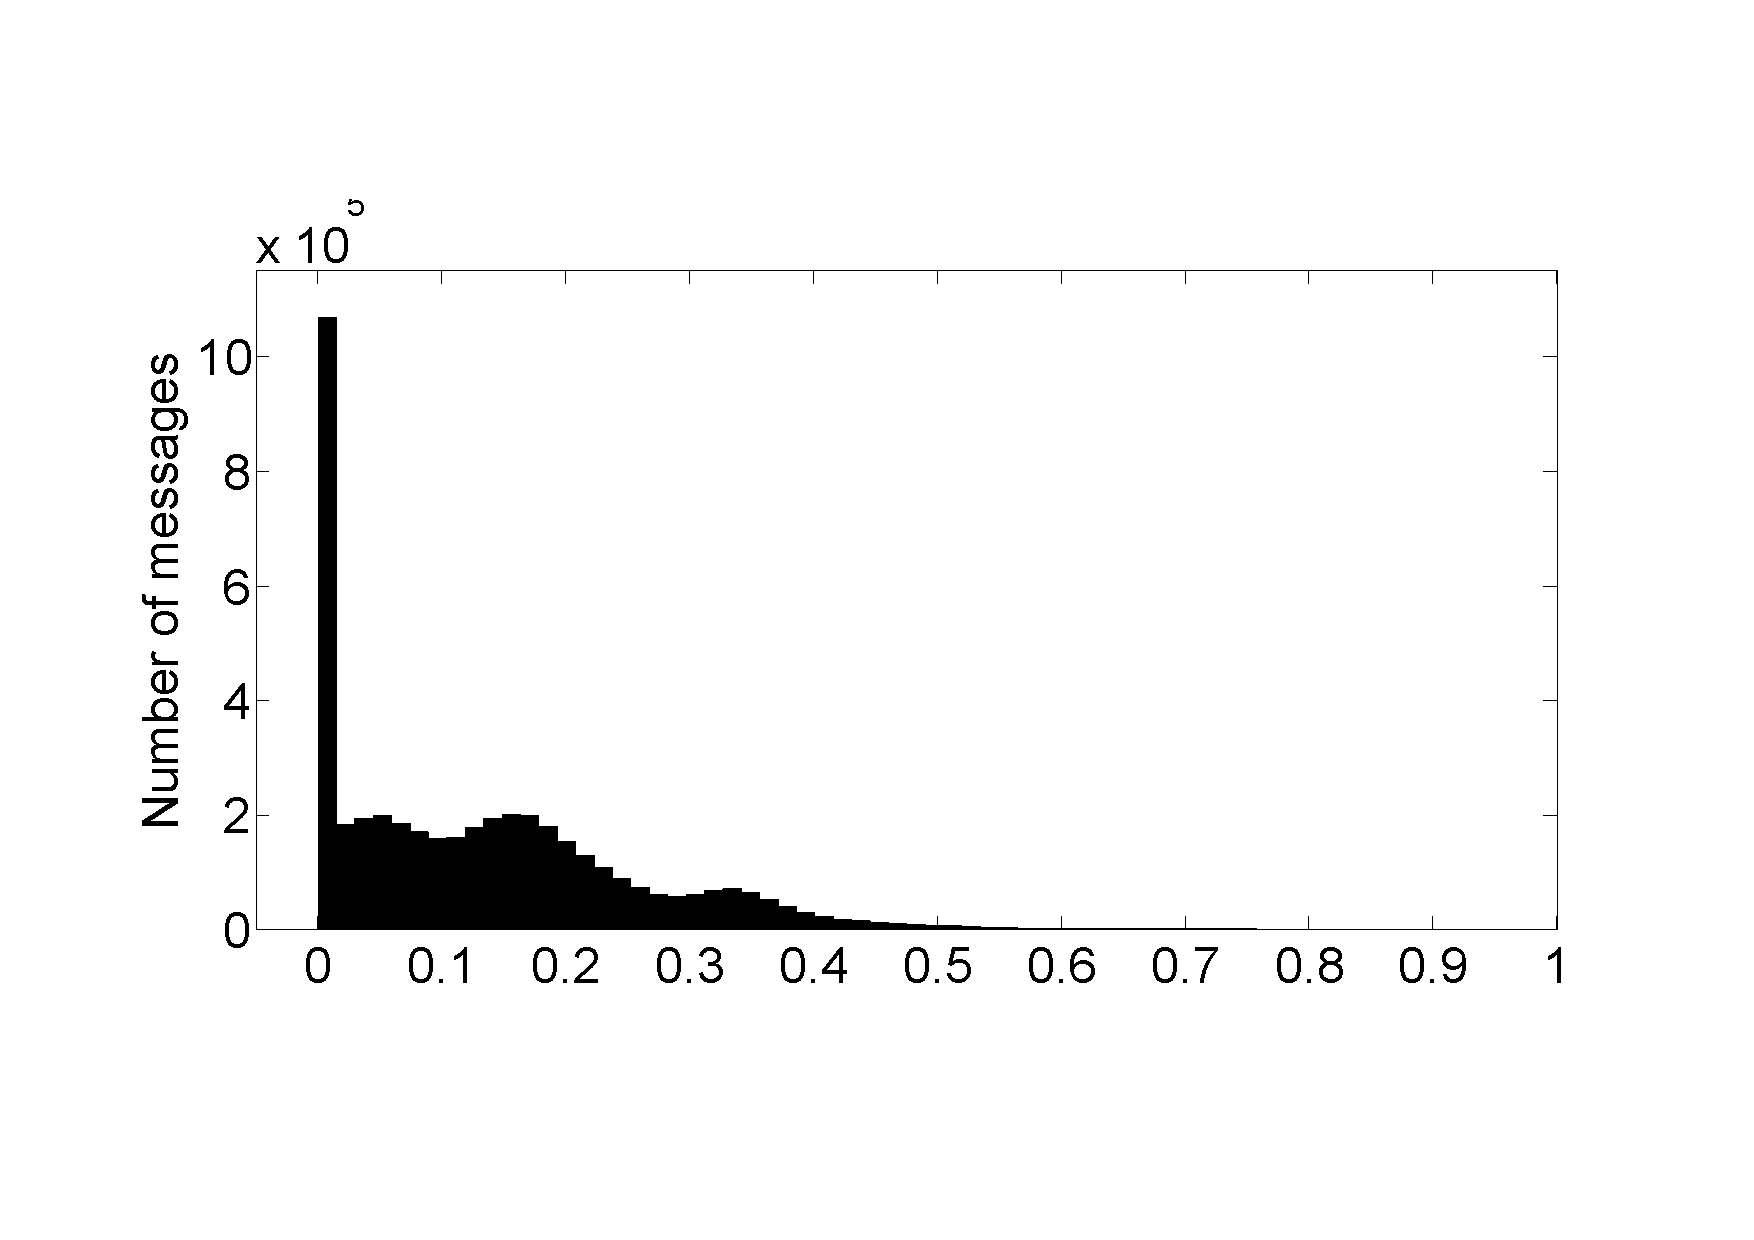
\includegraphics[clip=true, viewport=20mm 30mm 265mm 180mm, width=\columnwidth]{overall_get_ff}
 \caption{Overall retrieval responsiveness for safe or fast storage and fast retrieval}
 \label{fig_overall_get_ff}
\end{figure}
%
Figure \ref{fig_overall_get_ff} shows overall retrieval responsiveness for fast retrieval and safe or fast storage. The shape is similar to that of fast group retrieval in Figure \ref{fig_group_get_sf}, because in this case, fast retrieval returns the first result received. Since fast group retrieval is mostly faster then overlay retrieval, the overall retrieval distribution will closely match that of fast group retrieval.

\subsubsection{Parallel retrieval and safe or fast storage}
\begin{figure}[htbp]
 \centering
 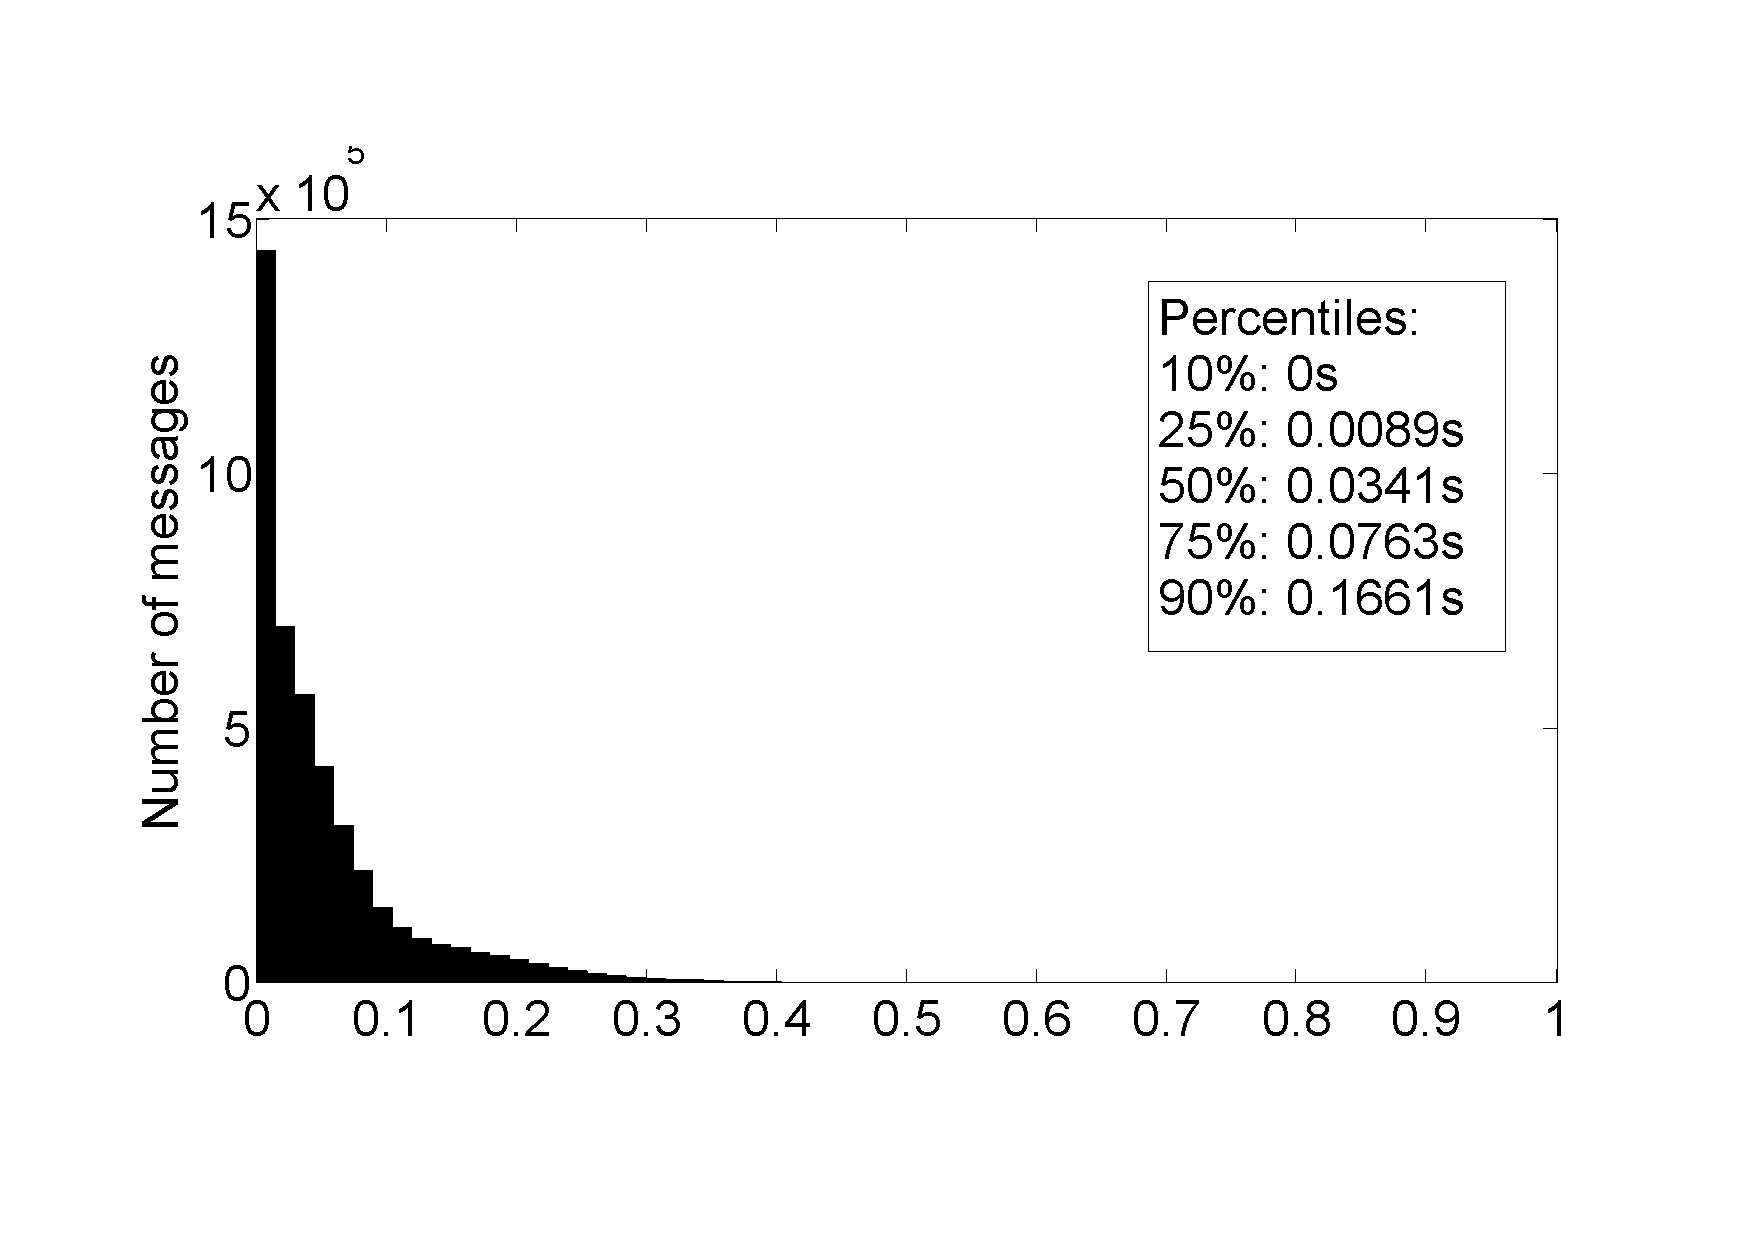
\includegraphics[clip=true, viewport=20mm 30mm 265mm 180mm, width=\columnwidth]{overall_get_fp}
 \caption{Overall retrieval responsiveness for fast storage and parallel retrieval}
 \label{fig_overall_get_fp}
\end{figure}
%
Figure \ref{fig_overall_get_fp} shows the overall retrieval responsiveness for parallel retrieval and safe or fast storage. Overall parallel retrieval mirrors parallel group retrieval, since parallel retrieval is faster than overlay retrieval and the first response is the one sent from the lower Pithos layers to peer logic.

\subsection{Conclusion}

In this section some responsiveness distributions were shown. The first reason was to enable the reader to not only compare mean performance values, but also range and shape. Secondly, it enables the highlighting of various structures and characteristics of storage and retrieval as they relate to certain quantities or mechanisms in Pithos, for examples timeouts. Thirdly, the distributions assist in verifying the correct working of Pithos. Especially when comparing the overall performance to the underlying group and overlay performance. It shows that Pithos is indeed a hybrid of those two storage types, but also that it is selecting the best quantities of the two. What this means is that any overlay can be selected and Pithos should perform better than the overlay.

\section{Performance for various group probabilities}
\label{group_probability_results}

The design of Pithos makes use of user groups and distance-based storage on a group layer, as stated in Sections \ref{grouping} and \ref{distance_based}. To be able to verify the actual performance of Pithos, it is therefore required to investigate Pithos's performance for various group probabilities. In the final P2P MMVE architecture, because of distance-based storage, it is assumed that the percentage of in-group requests will be much higher than that of out-of-group requests. This assumption is based on the fact that with group-based distance-based storage, the objects that are frequently of interest to the user will be stored in that user's group.

\subsection{Experimental setup}

\begin{itemize}
\item Because the exact probability that an object request will be for a group object is not yet known, a sweep is done for various group probabilities (the probability that a request is for a in-group object) to investigate the effect of group probability on Pithos's performance.
    
\item The ``low'' overlay is used for overlay storage. The low overlay was used to give a wider range of results from group storage to overlay storage.
 
 \item Fast  group storage is used. 
 
 \item Fast group retrieval is used.
 
 \item Six object replicas are stored.
 
 \item Nodes have mean lifetimes of 1800s.
 
 \item Objects have a TTL of 300s.
\end{itemize}

\subsection{Reliability}

\begin{figure}[htbp]
 \centering
 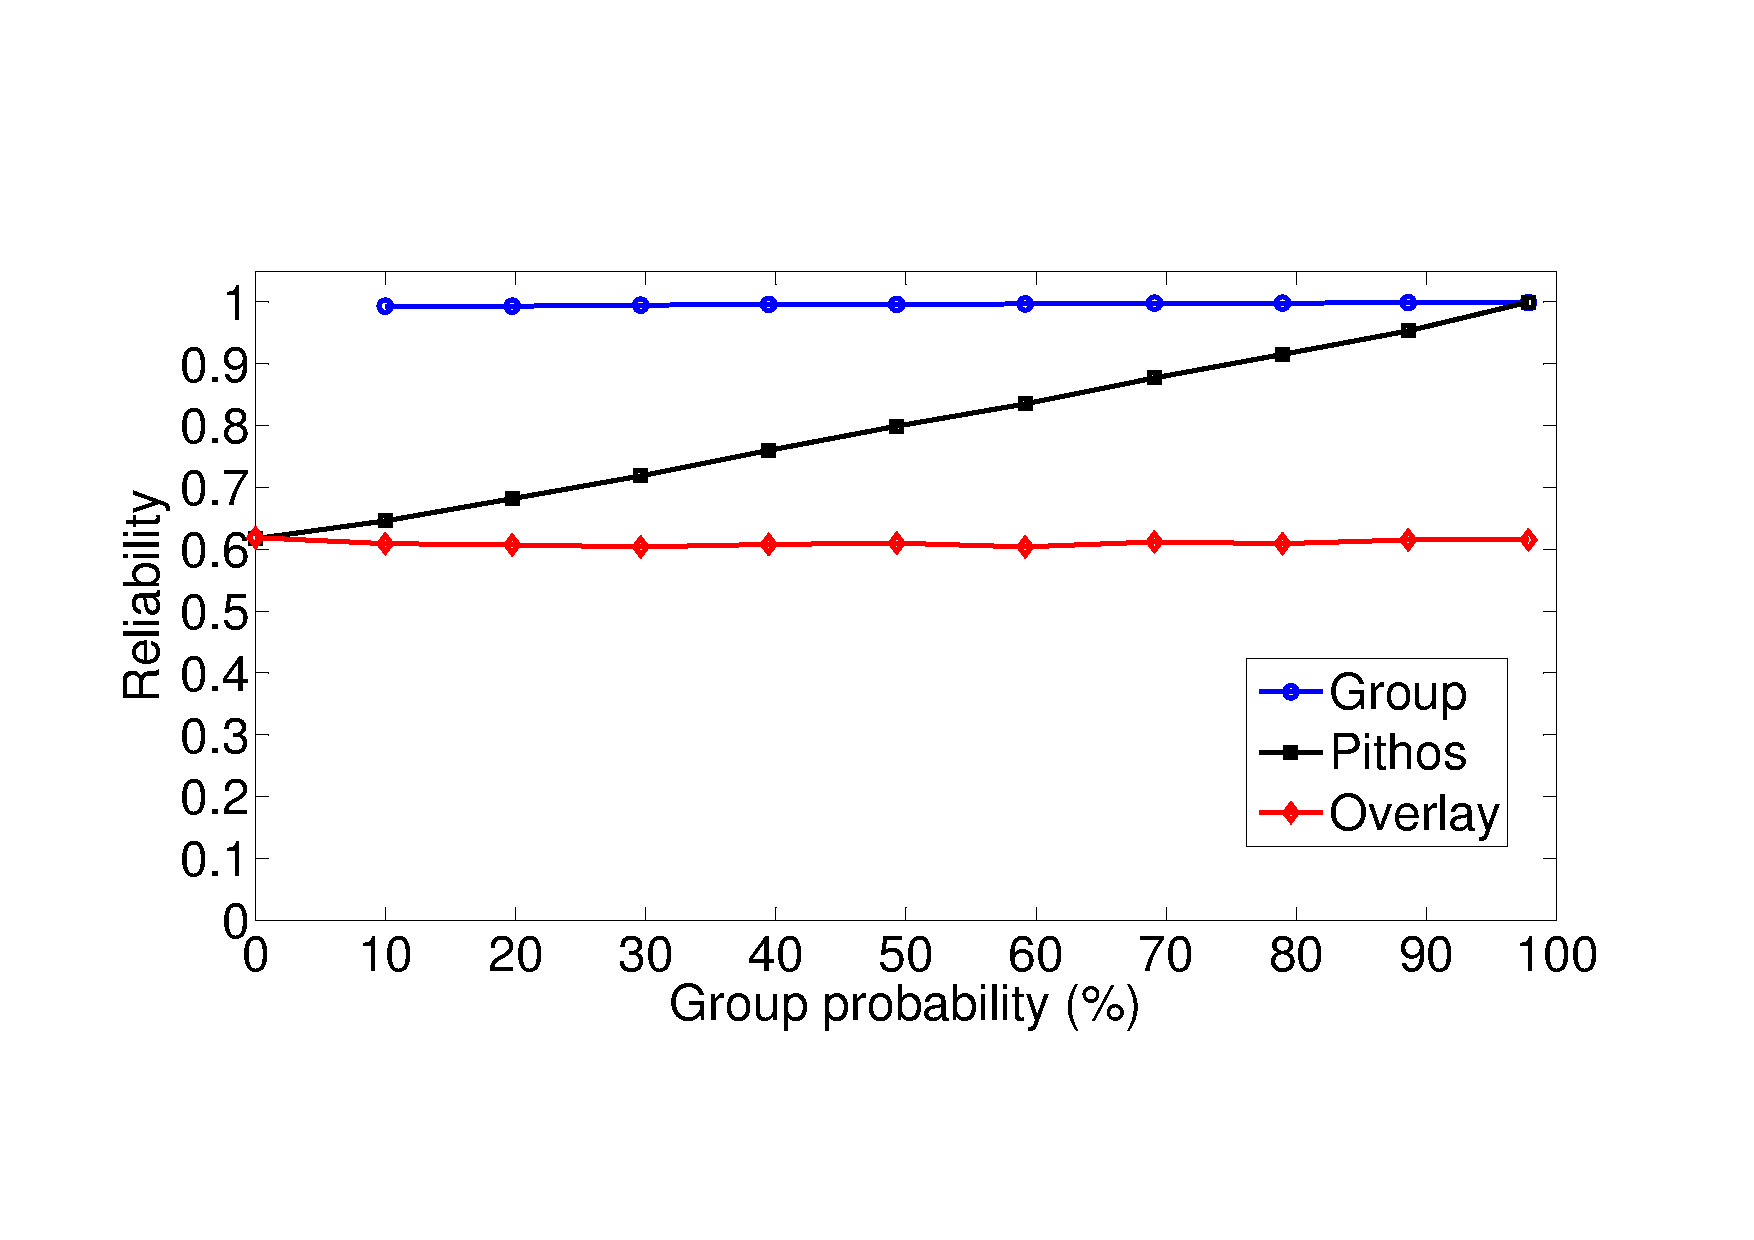
\includegraphics[clip=true, viewport=20mm 30mm 265mm 180mm, width=\columnwidth]{group_prob_rel}
 \caption{Reliability of Pithos, group storage and overlay storage for various group probabilities.}
 \label{fig_group_prob_rel}
\end{figure}
%
Figure \ref{fig_group_prob_rel} shows the effect group probability has on Pithos's overall reliability, compared with the underlying group storage and overlay storage reliabilities. The figure shows that the most reliable storage mechanism is group storage. It shows that group and overlay reliability are independent of the group percentage, which is as expected since the group storage and overlay storage modules are independent. Each request that is received from the higher layer (PithosTestApp) is relayed to both the DHT storage and group storage modules by the peer logic module.

When an object request is sent to group storage, the group storage module reports that there does not exist such a module in the group and the request is not handled. The only possible reply is then from the overly storage module. Figure \ref{fig_group_prob_rel} shows that the overall Pithos reliability is a linear combination of group storage and overlay storage, weighted by the group probability, or stated mathematically as:
%
\begin{equation}
R_{\textrm{Pithos}} = P_{\textrm{group}}R_{\textrm{group}} + (1-P_{\textrm{group}})R_{\textrm{overlay}},
\end{equation}
%
where $R_{\textrm{Pithos}}$ is the overall Pithos reliability, $R_{\textrm{group}}$ is the group reliability, $R_{\textrm{overlay}}$ and $P_{\textrm{group}}$ is the group probability.

This result shows that the reliability of Pithos varies linearly between overlay and group storage reliability as the group probability is varied. It should be noted that if a more reliable overlay was used, the medium or high configurations for example, the difference between group and overlay reliability is less. The low overlay configuration was just selected to better illustrate the linear relationship.

\subsection{Responsiveness}

\begin{figure}[htbp]
 \centering
 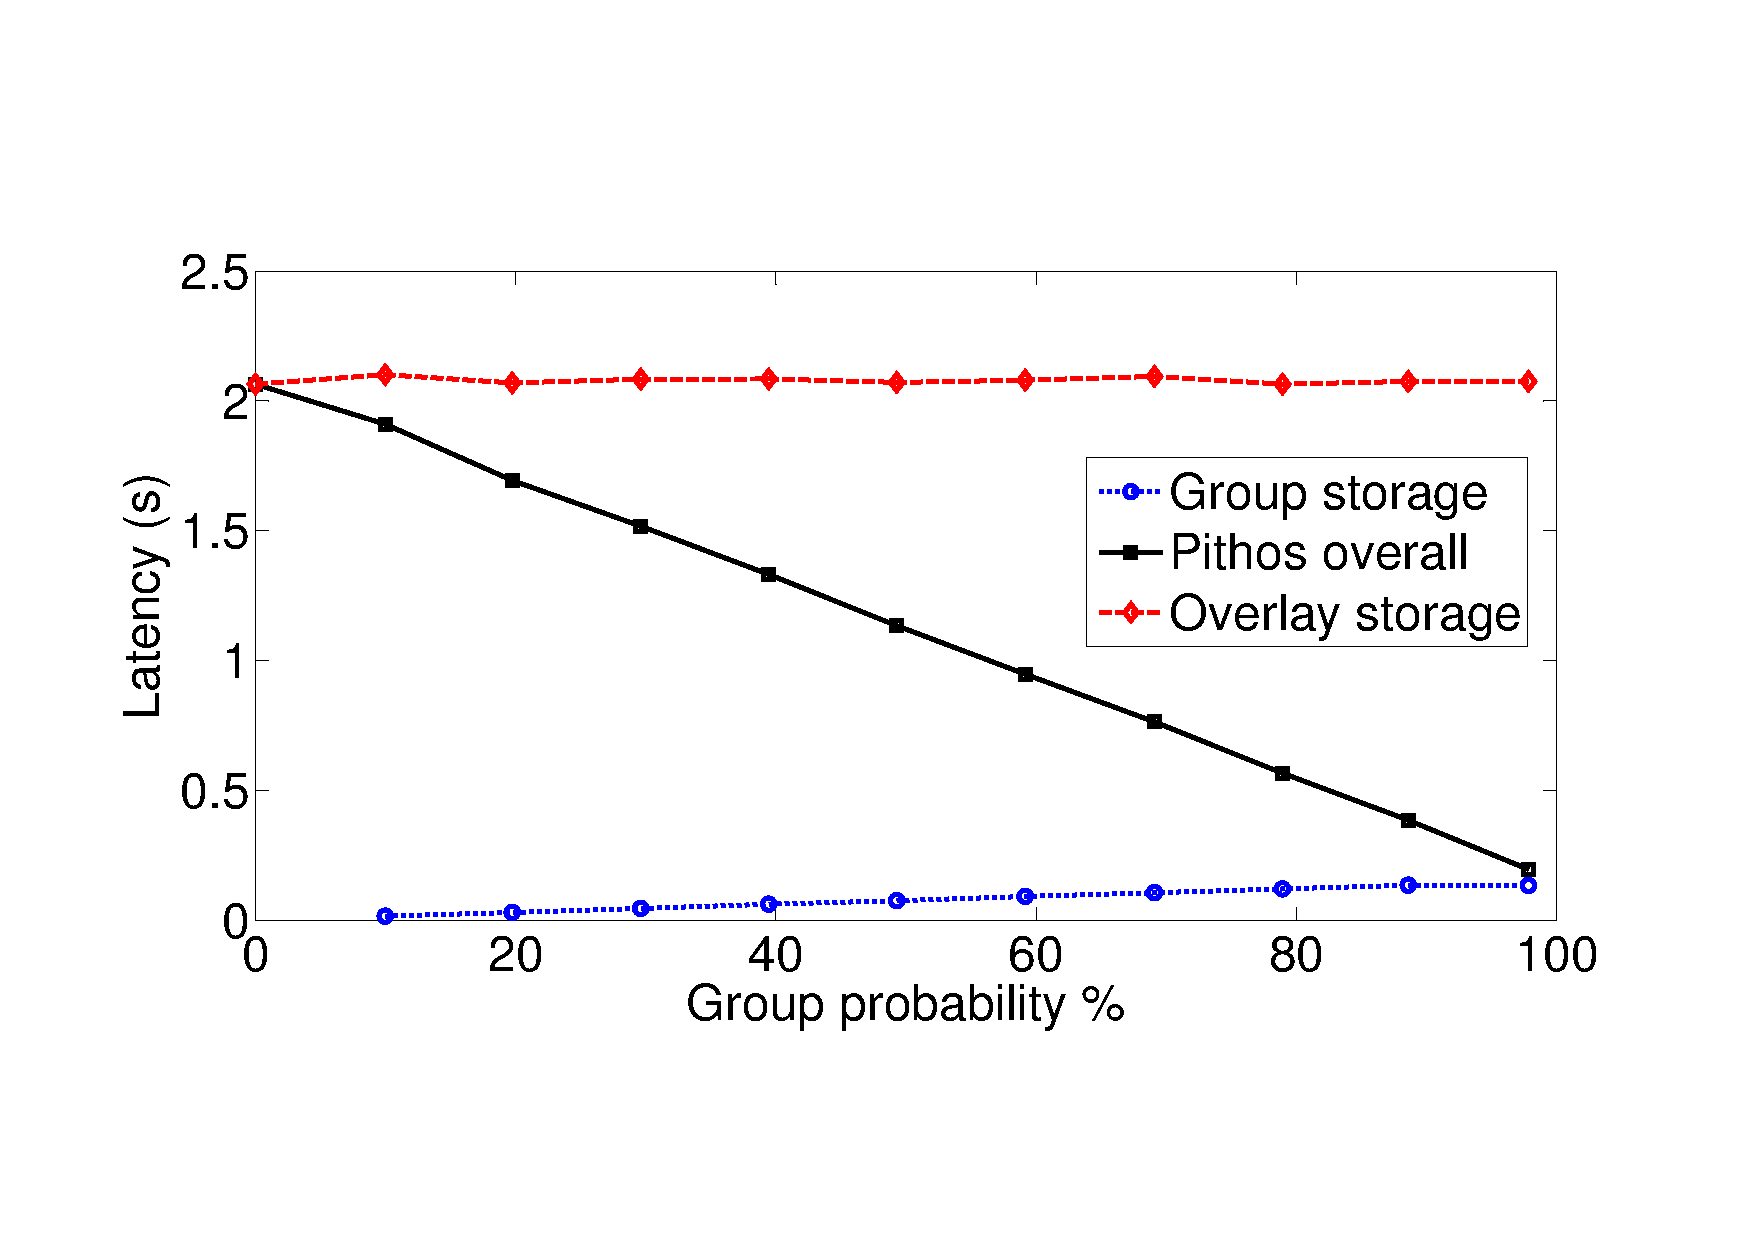
\includegraphics[clip=true, viewport=20mm 30mm 275mm 180mm, width=\columnwidth]{group_prob_resp}
 \caption{Responsiveness of Pithos, group storage and overlay storage for various group probabilities.}
 \label{fig_group_prob_resp}
\end{figure}
%
Figure \ref{fig_group_prob_resp} shows the responsiveness of Pithos compared with the underlying responsiveness of group and overlay storage. Take note that a lower value is preferred in this graph and that low latency is high responsiveness. As with the reliability, overall responsiveness is also shown to be a linear combination of group and overlay responsiveness.

An apparent anomaly is the group storage responsiveness that decreases with an increase in group probability. Recall that if a request is sent to group storage for an object not in the group, group storage immediately returns failure. The failure response is recorded as a response from group storage, even if this response is a failure.

The lower the group probability, the more failure responses are returned by group storage, which are returned instantly. It is these responses that decrease the mean group storage responsiveness for low group probabilities. When failure responses are ignored, group responsiveness remain constant at the value of 100\% group probability.

\subsection{Bandwidth}

\begin{figure}[htbp]
 \centering
 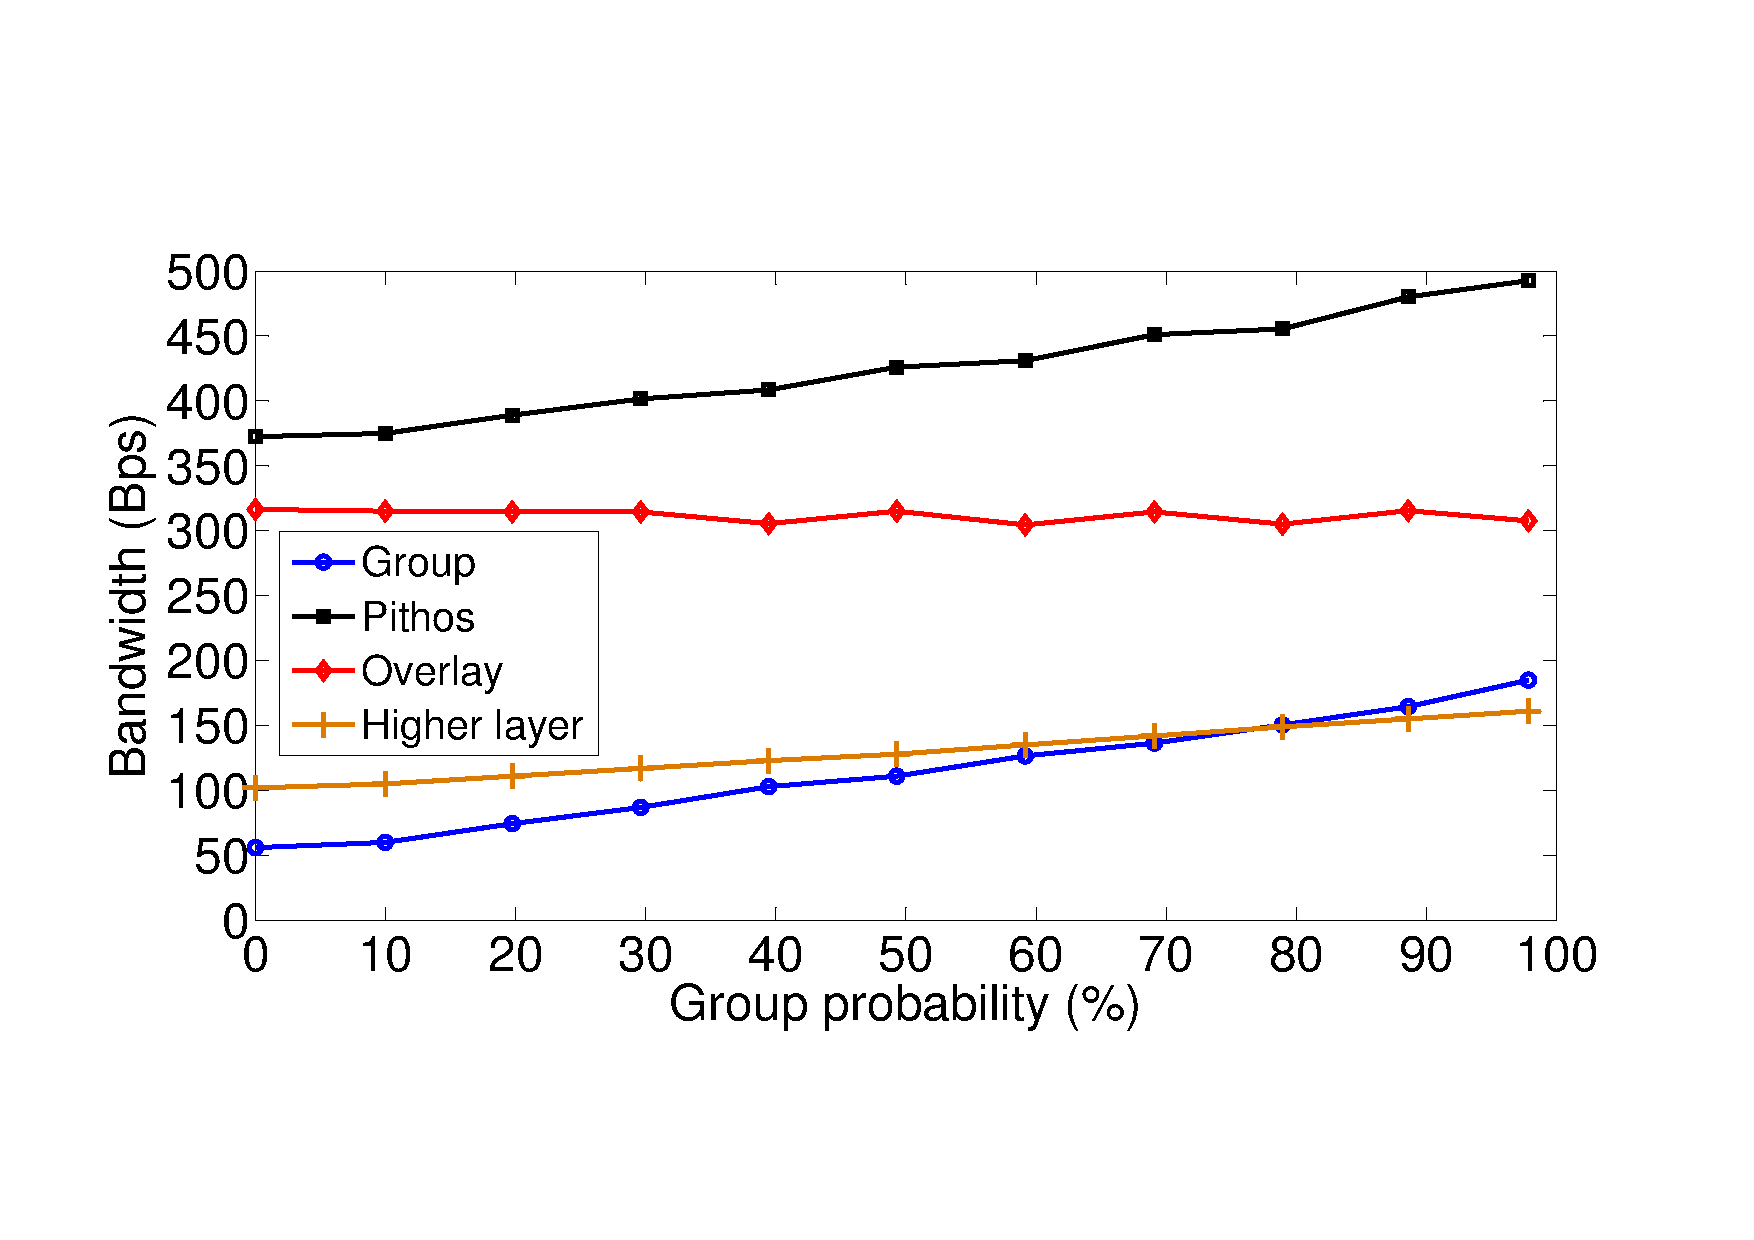
\includegraphics[clip=true, viewport=15mm 30mm 270mm 180mm, width=\columnwidth]{group_prob_bw}
 \caption{Bandwidth usage of Pithos, group storage and overlay storage for various group probabilities, as well as the bandwidth sent to, and received from Pithos.}
 \label{fig_group_prob_bw}
\end{figure}
%
Figure \ref{fig_group_prob_bw} shows the bandwidth requirements of Pithos in bytes per second (Bps). Pithos, group and overlay bandwidths show the mean of the inbound and outbound bandwidth. This was done, because the two values are similar and to make the graph more readable. Figure \ref{fig_group_prob_bw} also shows the underlying bandwidth requirements of group storage and overlay storage. To determine the actual overhead that Pithos requires, the graph also shows the amount of data that is sent to, and received from, Pithos, from and to the higher layer (PithosTestApp).

Figure \ref{fig_group_prob_bw} shows that overlay storage bandwidth remains constant, but that group storage bandwidth increases. Overlay storage remains constant, because no matter what the group probability is, the overlay storage is always queried for a data item and a data item is returned with the same probability (based on the reliability). Group storage, on the other hand, only returns data if the object exists within the group. Higher group probability means that more objects are requested from within the group, which means that group probability will return more objects and thereby use more data.

As shown, the overall Pithos bandwidth the the sum of the bandwidth required by group and overlay storage.

The data sent to Pithos is less than the data received from Pithos, because more retrieval requests are performed in the simulation than storage requests.

The graph shows that Pithos overhead is approximately 76\% of data in the network, where the majority of overhead is contributed by overlay storage.

\subsection{Conclusion}

This section reviews the performance of Pithos for various group probabilities and also shows the interaction between overlay and group storage in terms of reliability, responsiveness and bandwidth.

All all sections, what was seen was that for a low group probability, the characteristics of overlay storage are dominant and for high group probability, the characteristics of group storage are dominant. As previously stated, because of the distance-based storage design, high group probabilities are expected.

What was shown in this section is that overlay storage provides mediocre reliability for relatively high bandwidth requirements. This underpins the need for an overlay better suited to environments with network churn and improved lookup reliability. Before overlay efficiency can be improved, it is therefore important to create a grouping algorithm that has the highest possible group probability.

\section{Performance under object repair}
\label{repair_results}

%With TTL=1000

\subsection{Experimental setup}
\subsection{Reliability}
\subsection{Responsiveness}
\subsection{Bandwidth}
\subsection{Conclusion}

\begin{table}[htbp]
\centering
\begin{tabular}{|c|c|c|}
\hline
Repair   &Node lifetime& Data\\
         &     (s)     &in/out (Bps)\\
\hline
None     & 200         &     7/30\\
None     & 1000        &     5/135\\
None     & 1800        &     4/157\\
Leaving  & 200         &     7/49\\
Leaving  & 1000        &     5/136\\
Leaving  & 1800        &     4/158\\
Periodic & 200         &     7/53\\
Periodic & 1000        &     5/137\\
Periodic & 1800        &     4/157\\
\hline
\end{tabular}
\caption{Table showing the amount of data received and sent from and to the higher layer, for various repair profiles.}
\label{tab_repair_data}
\end{table}

\begin{table}[htbp]
\centering
\begin{tabular}{|c|c|c|c|c|c|}
\hline
Repair   &Node lifetime& Reliability  &  Responsiveness  &Group bandwidth&Overlay bandwidth  \\
         &     (s)     & retrieve     &  retrieve (s)    & in/out (Bps)  &  in/out (Bps)     \\
\hline
None     & 200         &    0.5437    &      1.430       &   133/92      &   876/891         \\
None     & 1000        &    0.9929    &      0.200       &   198/153     &   1157/1170       \\
None     & 1800        &    0.9987    &      0.157       &   191/162     &   1182/1195       \\
Leaving  & 200         &    0.8801    &      0.768       &   455/356     &   633/648         \\
Leaving  & 1000        &    0.9971    &      0.167       &   240/200     &   1161/1176       \\
Leaving  & 1800        &    0.9989    &      0.147       &   205/179     &   1182/1195       \\
Periodic & 200         &    0.9562    &      0.470       &   588/485     &   877/892         \\
Periodic & 1000        &    0.9971    &      0.167       &   251/209     &   1162/1176       \\
Periodic & 1800        &    0.9988    &      0.152       &   223/194     &   1182/1194       \\
\hline
\end{tabular}
\caption{Table showing the effect of network churn on the reliability and responsiveness of Pithos, for a fixed repair profile, fast storage and fast retrieval.}
\label{tab_repair_results}
\end{table}

\section{Reliability under malicious nodes}
\label{malicious_results}

What remains to be shown is Pithos's resistance to malicious peers when safe retrieval is used, as described in Section \ref{retrieve_implementation}.

Each object in Pithos has a double value attribute that is set to a random value when an object is created for the simulation. The value of the object is stored in PithosTestApps's global object list. It should be noted that for simulation purposes, an object's size is not related to its content. An object's size is set using a random distribution and this is the value used to compute transmission bandwidth and latency.

Whenever a malicious node receives a retrieval request it replies with a modified version of the requested object. The object is modified by modifying the object value. An object is assigned a uniformly random value by a malicious node. Because of the way objects are altered, we implicitly assume that there exists no collusion in the network. When PithosTestApp receives a requested object, it checks that object against the global object list to determine whether the correct object was received. PithosTestApp then records Pithos's reliability.

Pithos selects the object that is the same in a majority of responses and sends it to the higher layer. If no object has a majority, a failure response is sent to the higher layer.

\subsection{Experimental setup}

\begin{itemize}
\item The percentage of users that are malicious is varied from 0.0 to 1.0 in steps of 0.125.
 
\item Fast group storage is used.

\item Fast and safe group retrieval are compared.

\item For the safe retrieval case, six objects are retrieved.
  
\item A comparison of safe retrieval is performed by first retrieving four of the six stored replicas and then retrieving six.
    
\item Node lifetimes are set to 1800s mean.

\item Object TTL is set to 300s.
\end{itemize}

\subsection{Results}
\begin{figure}[htbp]
 \centering
 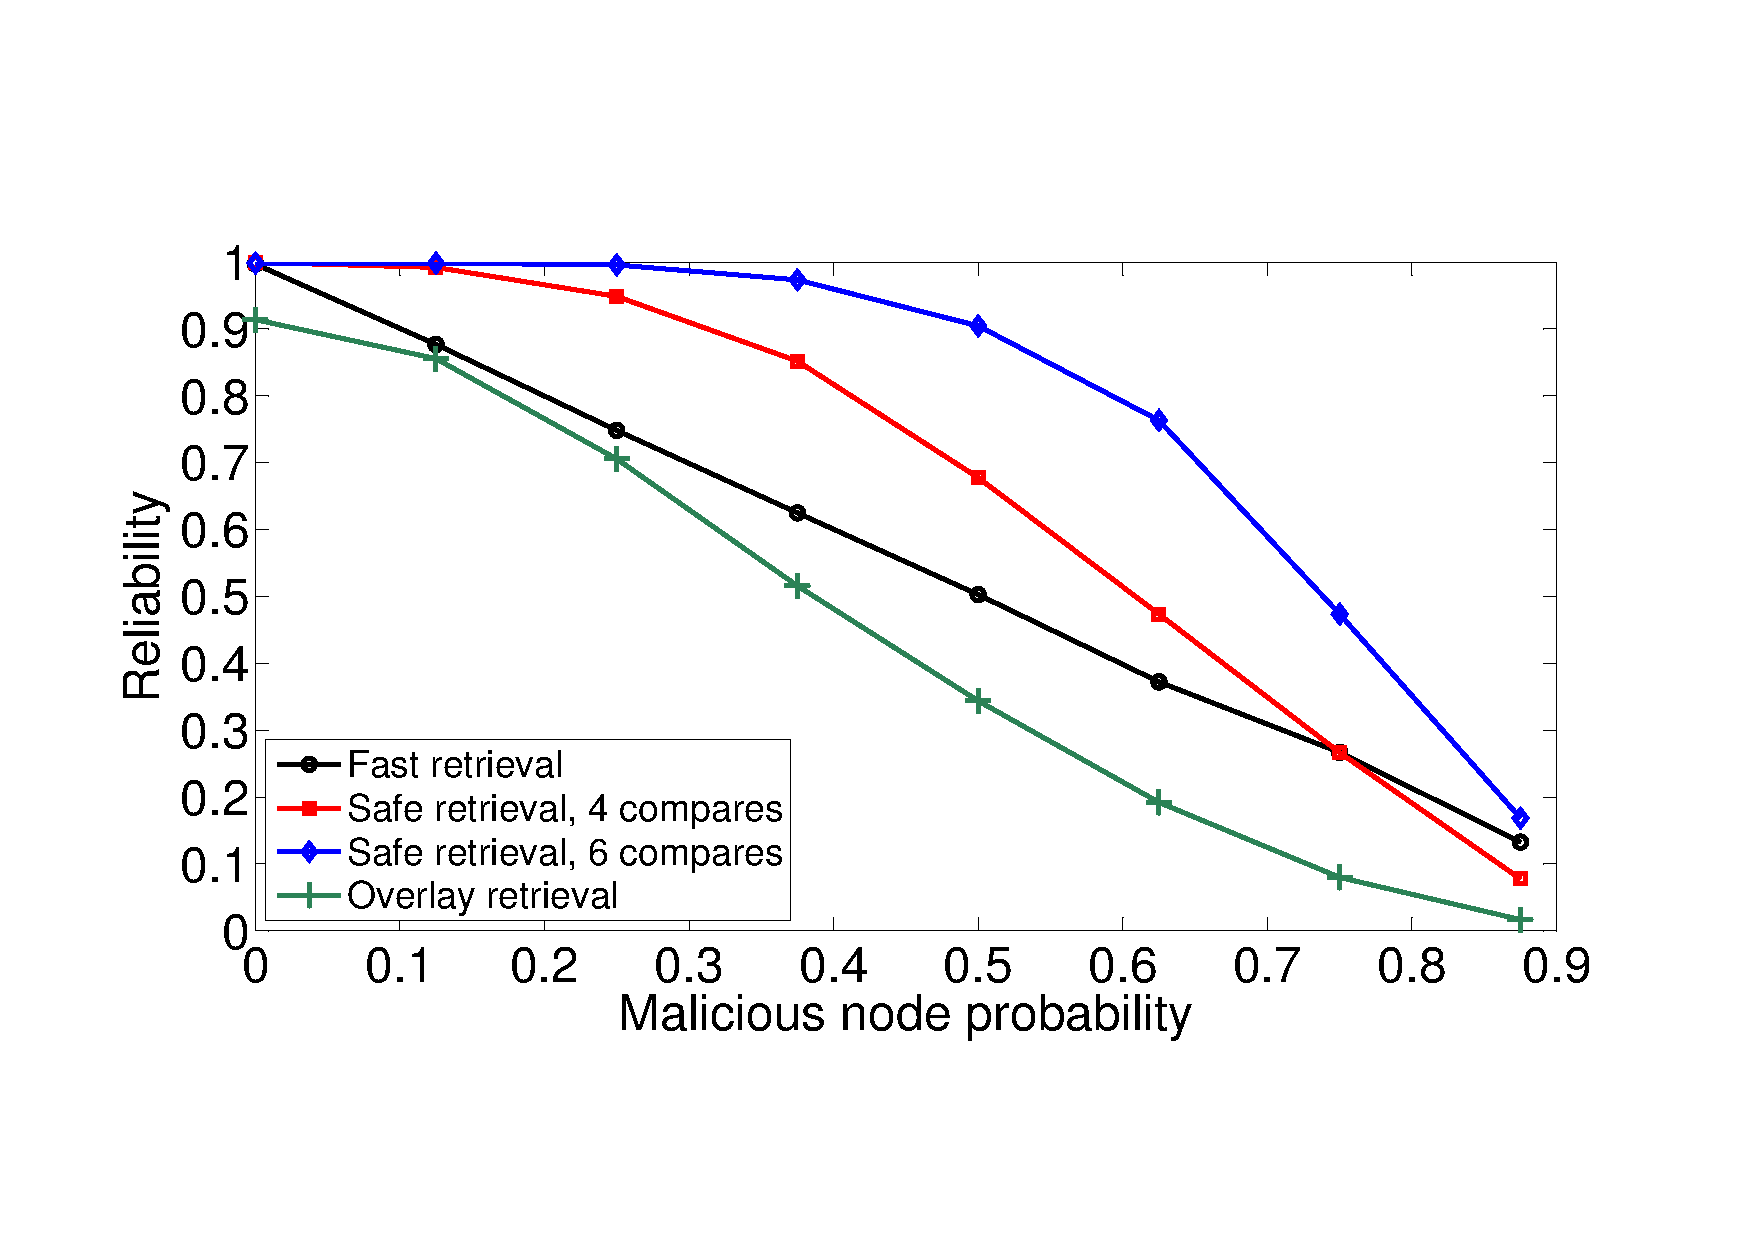
\includegraphics[clip=true, viewport=20mm 30mm 270mm 175mm, width=\columnwidth]{malicious_nodes_rel}
 \caption{Reliability of various Pithos retrieval schemes for varying factors of malicious node probability.}
 \label{fig_malicious_nodes_rel}
\end{figure}
%
Figure \ref{fig_malicious_nodes_rel} shows Pithos's reliability as a function of the percentage of malicious users in the network for both the fast retrieval and safe retrieval schemes. The fast retrieval reliability is almost the same as the malicious user percentage. System reliability for fast retrieval is the product of the malicious user factor and the system reliability under no malicious users.

The reason for this direct relationship is because the probability of an object retrieval being corrupted in the network is equal to the probability of a peer being malicious, since a malicious peer corrupts all objects returned and a non-malicious peer corrupts none of the objects returned. The overall probability is then the probability that an object retrieval would have succeeded if no malicious nodes were present, multiplied by the probability of nodes being malicious.

Figure \ref{fig_malicious_nodes_rel} also shows the improvement received from using safe retrieval. The curve shows that safe retrieval provides greater benefit for smaller factors of malicious nodes. As soon as the majority of objects are corrupted, object reliability drops significantly.

The figure also shows improved reliability, when more received objects are compared to select a majority. Retrieving more objects for comparison will, however, increase bandwidth requirements. Bandwidth increases in line with that shown in Section \ref{bandwidth_requirements}, because safe retrieval is parallel retrieval, but for an additional compare operation. It should be noted that more retrievals than compares may be performed to increase responsiveness at the cost of additional bandwidth.

An interesting situation arises, where safe retrieval reliability drops below fast retrieval reliability. When a majority can no longer be identified by safe retrieval, a failure response is sent up. This is as opposed to fast retrieval that sends any object received. It is possible the the object that was selected by fast storage was not maliciously altered, but also not in the majority. In this scenario, fast retrieval will sometimes send objects to the higher layer that were correct, where safe storage just responded with failure, because it couldn't be sure. Because in practice, the higher layer will not know whether an object is corrupted or not, it seemed more prudent to only send objects to the higher layer where Pithos was reasonably sure the object was unaltered.

\subsection{Conclusion}

The section shows that Pithos's safe retrieval mechanism can be used to increase reliability under malicious users at the cost of responsiveness and bandwidth. With malicious users usually present in a virtual world, this cost is always acceptable. During the lifetime of the virtual world, it is important to monitor that malicious user percentage, to determine how parameters, such as number of retrieve requests and number of compares, should be adjusted to combat the threat while minimising bandwidth and maximising responsiveness.

In practice, a low malicious node factor is expected, since it is assumed that cheaters are in the minority. If the virtual world has a majority of cheaters, it will most likely not be sustainable.

\section{Object distribution (fairness)}

One of the key reasons objects are distributed amongst groups is to achieve storage fairness. As described in Section \ref{fairness_requirement}, fairness is required to ensure that all peers contribute equally to the P2P network.

\begin{figure}[htbp]
 \centering
 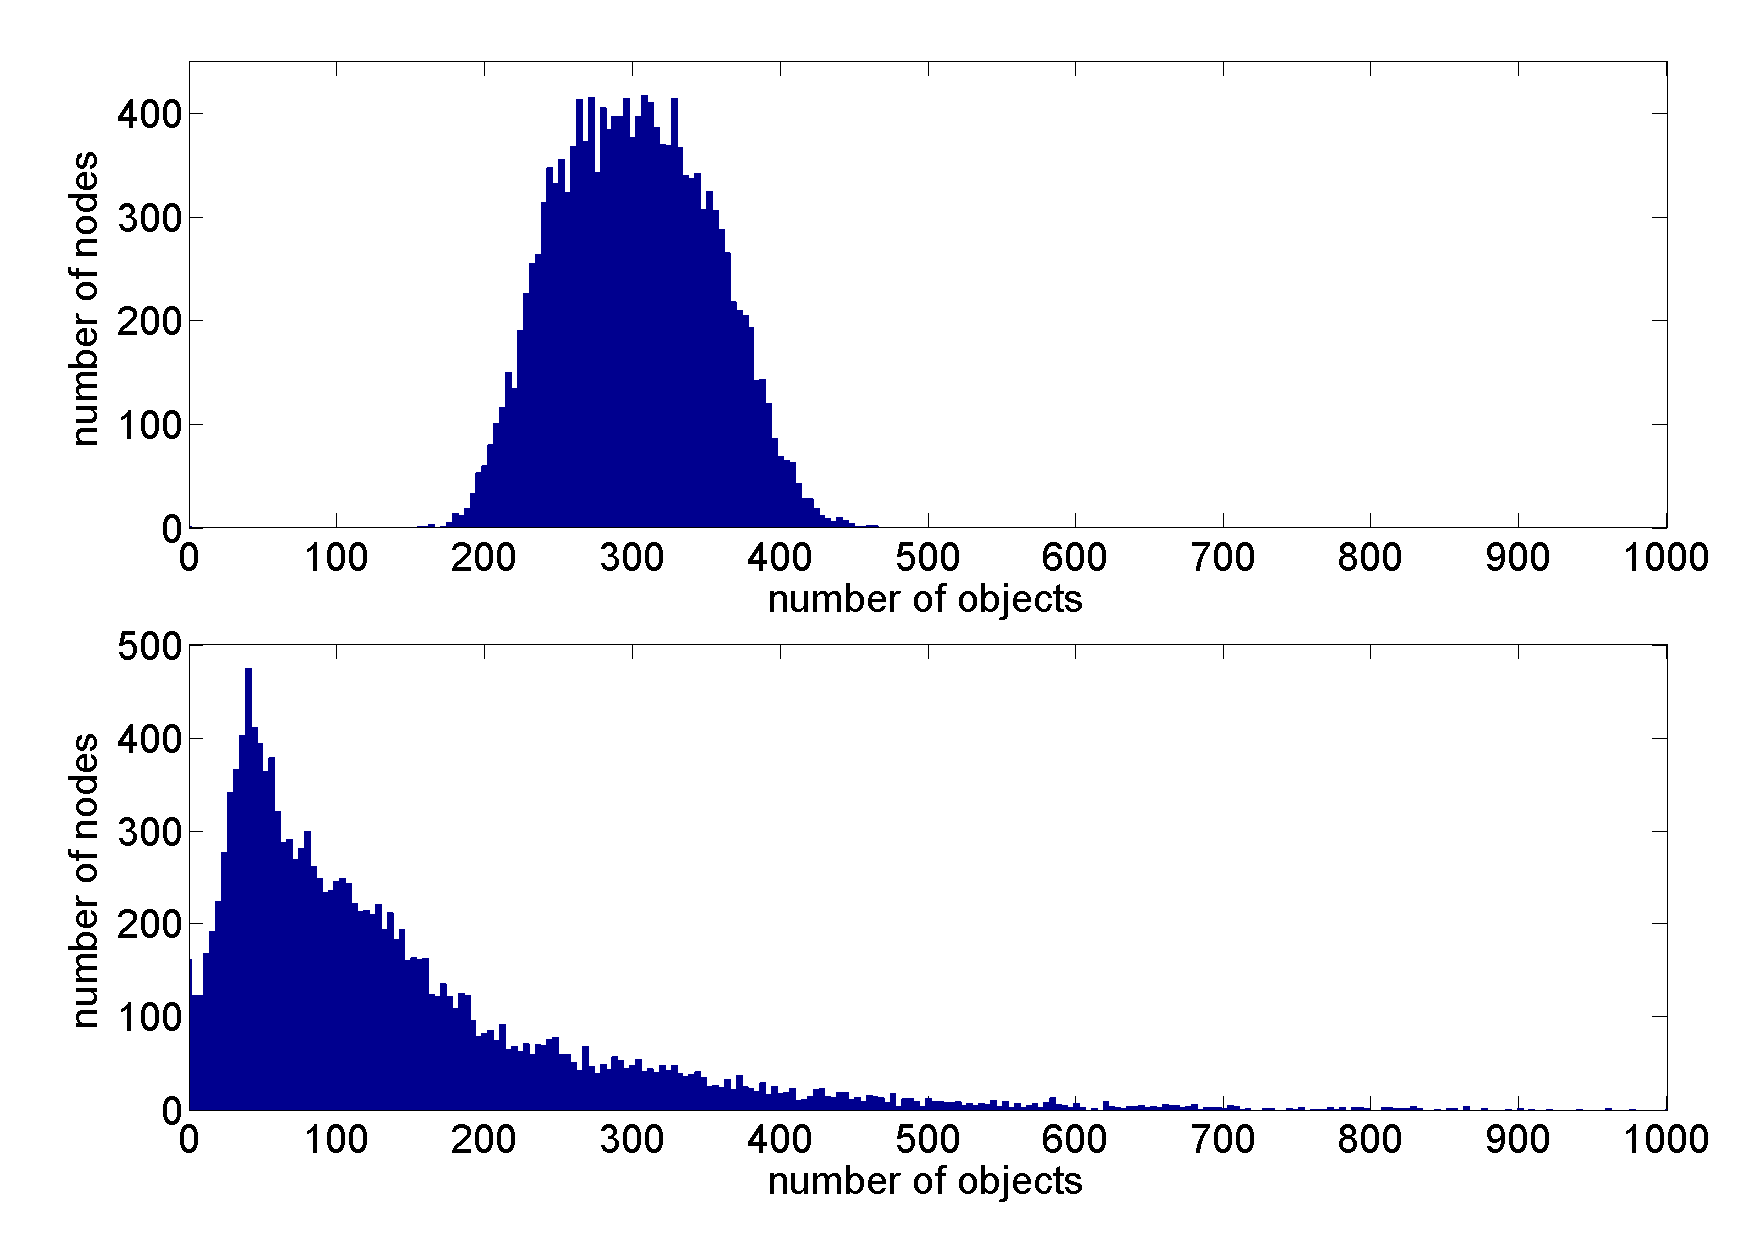
\includegraphics[clip=true, viewport=1cm 0.5cm 28.5cm 20cm, width=\columnwidth]{RootRepOverlayObjects}
 \caption{Top: Distribution showing the number of peers that store a certain number of group objects. Bottom: Distribution showing the number of peers that store a certain number of overlay objects.}
 \label{fig_group_overlay_objects}
\end{figure}
%
To evaluate the fairness, we evaluate the standard deviation of the number of objects stored per peer. Figure \ref{fig_group_overlay_objects} (top) shows the distribution of group objects over nodes in the network. The figure shows how many nodes store how many objects. The distribution has a mean and standard deviation of 302 and 51 objects per node respectively.

Figure \ref{fig_group_overlay_objects} (bottom) shows the distribution of overlay objects in Pithos with a mean and standard deviation of 153 and 189 objects per node respectively. Comparing the standard deviations of group storage to overlay storage, it appears that group storage is fairer than overlay storage.

\begin{figure}[htbp]
 \centering
 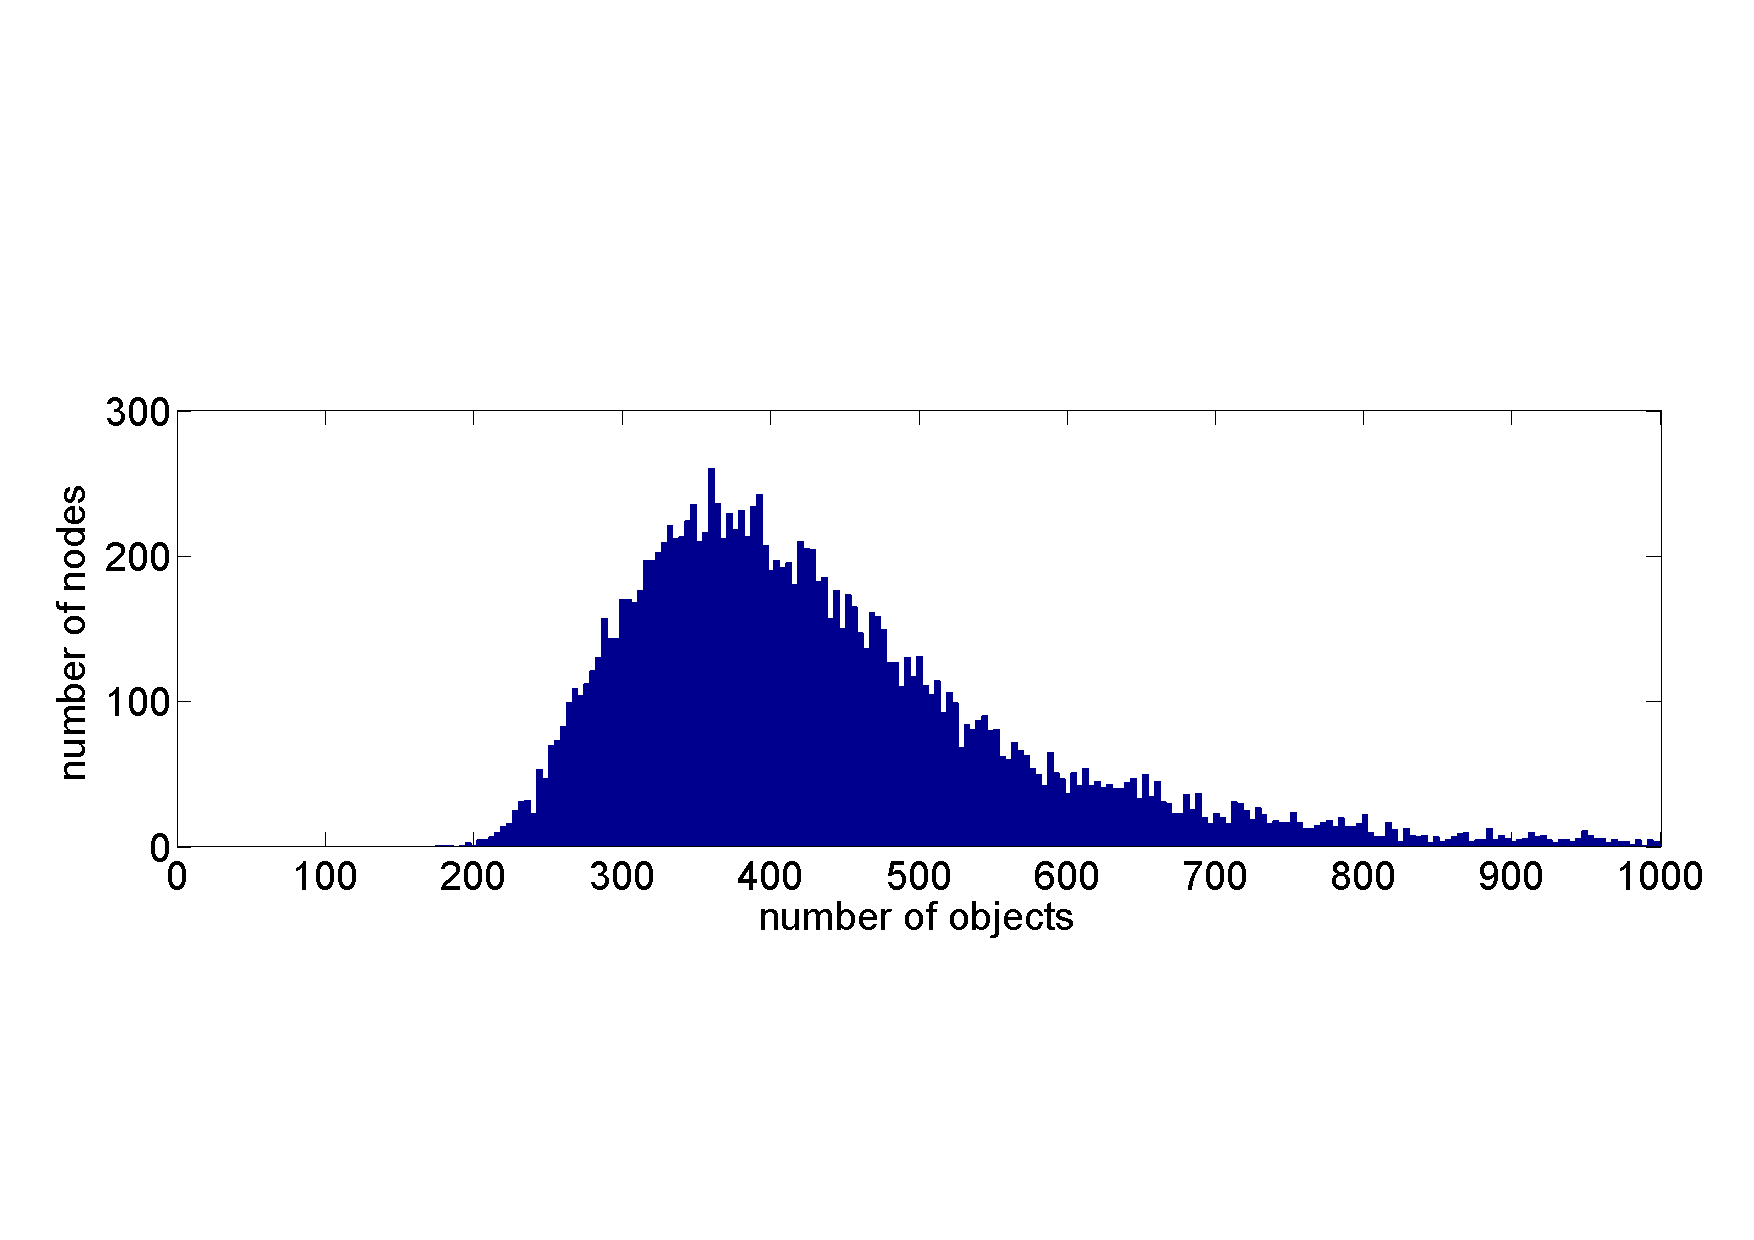
\includegraphics[clip=true, viewport=1cm 5cm 29cm 14.5cm, width=\columnwidth]{Objects}
 \caption{Combined object number distribution}
 \label{fig_objects}
\end{figure}
%
Figure \ref{fig_objects} shows the combined object distribution of Pithos, with a mean and standard deviation of 453 and 200 objects per node respectively. This shows that the fairness of Pithos is currently dominated by the fairness of the overlay and that Pithos is as fair as overlay storage.

What should be concluded from this section is that there does no exist a minority of peers in Pithos that store the majority of the data. All peers are required to contribute to the P2P network.

\section{Conclusion}

This section initially showed the storage and retrieval performance of Pithos, without taking into account group probability, object repair or malicious nodes. Fast storage was found to be sufficiently reliable for the large responsiveness gain it added. It was found that parallel storage are both more responsive and reliable than fast storage at the cost of additional bandwidth.

Overlay storage was found to be less reliable than initially thought, when taking into account its required bandwidth. Overlay storage is, however, the only way in which a peer may acquire data from outside of its group.

The responsiveness distributions for Pithos were also presented, along with a discussion of the results. The distributions verified the methods used to implement the store and retrieve mechanisms and also showed how the underlying group and overlay storage modules relate to the overall storage performance.

It was discussed that it is important to take group probability into account when evaluating Pithos performance. By varying the group probability, it was shown that the overall performance is a weighted average of the underlying group and overlay performances.

The effect of repair was shown by evaluating Pithos for various repair methods with varying node lifetimes. It was found that repair significantly increases reliability when the expected node lifetimes are small, compared to the object TTL. Repair is not required, if node lifetimes are large, compared to the object TTL.

Finally, it was shown that all peers in Pithos are required to contribute storage space to the network.
